%% Appendix section: Expert Interviews, Series Overview.
%% Included from tese.tex via %% Appendix section: Expert Interviews, Series Overview.
%% Included from tese.tex via %% Appendix section: Expert Interviews, Series Overview.
%% Included from tese.tex via %% Appendix section: Expert Interviews, Series Overview.
%% Included from tese.tex via \input{ApeA/expert_interviews_overview}.
%% Consolidates the session metadata, interviewee attribution, dimension
%% coverage, and saturation-axis status of the fifteen interview reports.

\section{Series overview}
\label{sec:interviews-overview}

This chapter presents the fifteen expert interview reports of the verification phase. The methodology, the seven-question protocol, and the analysis framework are consolidated in Appendix~\ref{ape:methodology}. All sessions were remote synchronous video calls, recorded and transcribed, with verbal consent captured on record, and all were conducted in Brazilian Portuguese: quotations in the per-interview sections preserve the original wording, followed by an English translation for the reader.

This overview consolidates the descriptive information that is common to every report: session metadata (Table~\ref{tab:interviews-metadata}), interviewee attribution (Table~\ref{tab:interviews-attribution}), coverage of the four evaluation dimensions (Figure~\ref{fig:interviews-dimensions}), and the cross-series status of the five saturation axes (Figure~\ref{fig:interviews-axes}). The per-interview sections that follow keep the analytical content of each session: the three strongest themes, the verbatim quote worth preserving, the coded findings with their literature-gap mapping, the post-interview questionnaire findings, the session-specific limitations, the contributions to the conclusions chapter, and a concluding remark.

\subsection*{Session metadata}

Table~\ref{tab:interviews-metadata} records the date and the total recording length of each session.

\begin{longtable}{c l l}
\caption{Session metadata of the fifteen interviews.}
\label{tab:interviews-metadata}\\
\toprule
\textbf{Interview} & \textbf{Date (2026)} & \textbf{Recording} \\
\midrule
\endhead
\bottomrule
\endfoot
01 & 29 May & approx.\ 99 min \\
02 & 1 June & approx.\ 68 min \\
03 & 1 June & approx.\ 50 min \\
04 & 1 June & approx.\ 71 min \\
05 & 2 June & approx.\ 62 min \\
06 & 2 June & approx.\ 45 min \\
07 & 3 June & approx.\ 80 min \\
08 & 5 June & approx.\ 58 min \\
09 & 6 June & approx.\ 76 min \\
10 & 8 June & 56 min \\
11 & 8 June & 65 min \\
12 & 8 June & approx.\ 42 min \\
13 & 10 June & approx.\ 46 min \\
14 & 9 June & 37 min \\
15 & 9 June & approx.\ 29 min \\
\end{longtable}

Four sessions declared an analytical cutoff, the timestamp after which the conversation leaves research-relevant content; material after the cutoff does not appear in any derived artifact. The excluded segments are administrative or post-closing conversation:

\begin{enumerate}[itemsep=8pt,topsep=2pt]
  \item \emph{Interview 01, cutoff at 01:14:43.} A confirmation-letter discussion and employer-proprietary tool demos.
  \item \emph{Interview 02, cutoff at 01:07:25.} A product brainstorm derived from the maturity matrix discussion.
  \item \emph{Interview 03, cutoff at 00:49:40.} Defense logistics and prior-interview commentary.
  \item \emph{Interview 09, cutoff at 01:14:00.} Scheduling updates without analytical material.
\end{enumerate}

The remaining eleven sessions were research-relevant in full.

\subsection*{Interviewee attribution}

Table~\ref{tab:interviews-attribution} consolidates the attribution of the fifteen participants under the \emph{Interviewee N} scheme declared in Appendix~\ref{ape:methodology}. Personal identifiers are withheld in all cases, and the reports disclose the employment context at three levels: Interviews 01 to 07 name the industry but not the employer, Interviews 08, 10, 11, and 12 name previous employers and keep the current one undisclosed, and Interviews 09, 13, 14, and 15 withhold the organization entirely (the three public-sector participants work at a Brazilian state-owned information technology company, named only by category).

\begin{longtable}{c p{6.0cm} p{4.6cm} c}
\caption{Interviewee attribution across the series.}
\label{tab:interviews-attribution}\\
\toprule
\textbf{Interview} & \textbf{Role and context} & \textbf{Education} & \textbf{XP (yrs)} \\
\midrule
\endhead
\bottomrule
\endfoot
01 & Principal Software Engineer, U.S.\ telecommunications & BSc Information Technology & 16 \\
02 & Senior Engineering Manager, U.S.\ SaaS (home services) & Dipl\^ome d'Ing\'enieur, ENSIIE (France) & 15 \\
03 & CTO across Brazilian startups & BSc Information Technology & 14 \\
04 & Engineering Manager, Australian software company; former consultant & not declared & 15 \\
05 & Principal Software Engineer, Brazilian edtech & PhD student, Software Engineering & 17 \\
06 & Adjunct professor, federal Brazilian university & PhD Computer Science (2016) & n/d \\
07 & Engineering Manager, Brazilian fintech & BSc Information Systems & 12 \\
08 & Principal Software Engineer, formerly at Shopify & Engineering degree & 10+ \\
09 & Software engineer, distributed and modular monolith systems & Dipl\^ome d'Ing\'enieur, \'Ecole Polytechnique; BEng Poli-USP & 4 \\
10 & Senior Software Engineer, formerly at GitHub and Red Hat & Engineering degree & 14 to 15 \\
11 & Software engineer, formerly at Samsung SRBR, Ita\'u, Viva Real & MSc Computer Science, UFAM & 10+ \\
12 & Backend Software Engineer, formerly at VR Benef\'icios and Ambev & Technologist, Systems Analysis, IFSP & 7 \\
13 & Engineering Manager, state-owned IT company (public sector) & MSc UFMG; doctoral student & 13 \\
14 & Software Engineer, state-owned IT company (public sector) & BSc Computer Science, UniBH & 10 \\
15 & Systems Analyst, state-owned IT company (public sector) & Technologist, Systems Analysis, Una & 13 \\
\end{longtable}

The profile categories tracked across the series are eleven industry practitioners, three mixed industry-and-academic profiles (Interviews 05, 11, and 13), and one academic researcher (Interview 06). The sample covers Brazilian, Australian, French, and United States contexts, with years of professional experience from four to seventeen.

\subsection*{Coverage of the four evaluation dimensions}

Figure~\ref{fig:interviews-dimensions} shows how thoroughly each session covered the four evaluation dimensions: D1 Architectural Design, D2 Operational Fit, D3 Organizational Alignment, and D4 Guideline Orientation. The cells use five markers: \emph{D} for covered with depth, \emph{B} for covered with breadth or covered more briefly, \emph{O} for addressed organically (the participant raised the dimension without prompting), \emph{I} for addressed implicitly or indirectly, and \emph{NA} for not addressed.

\begin{figure}[htb]
  \centering
  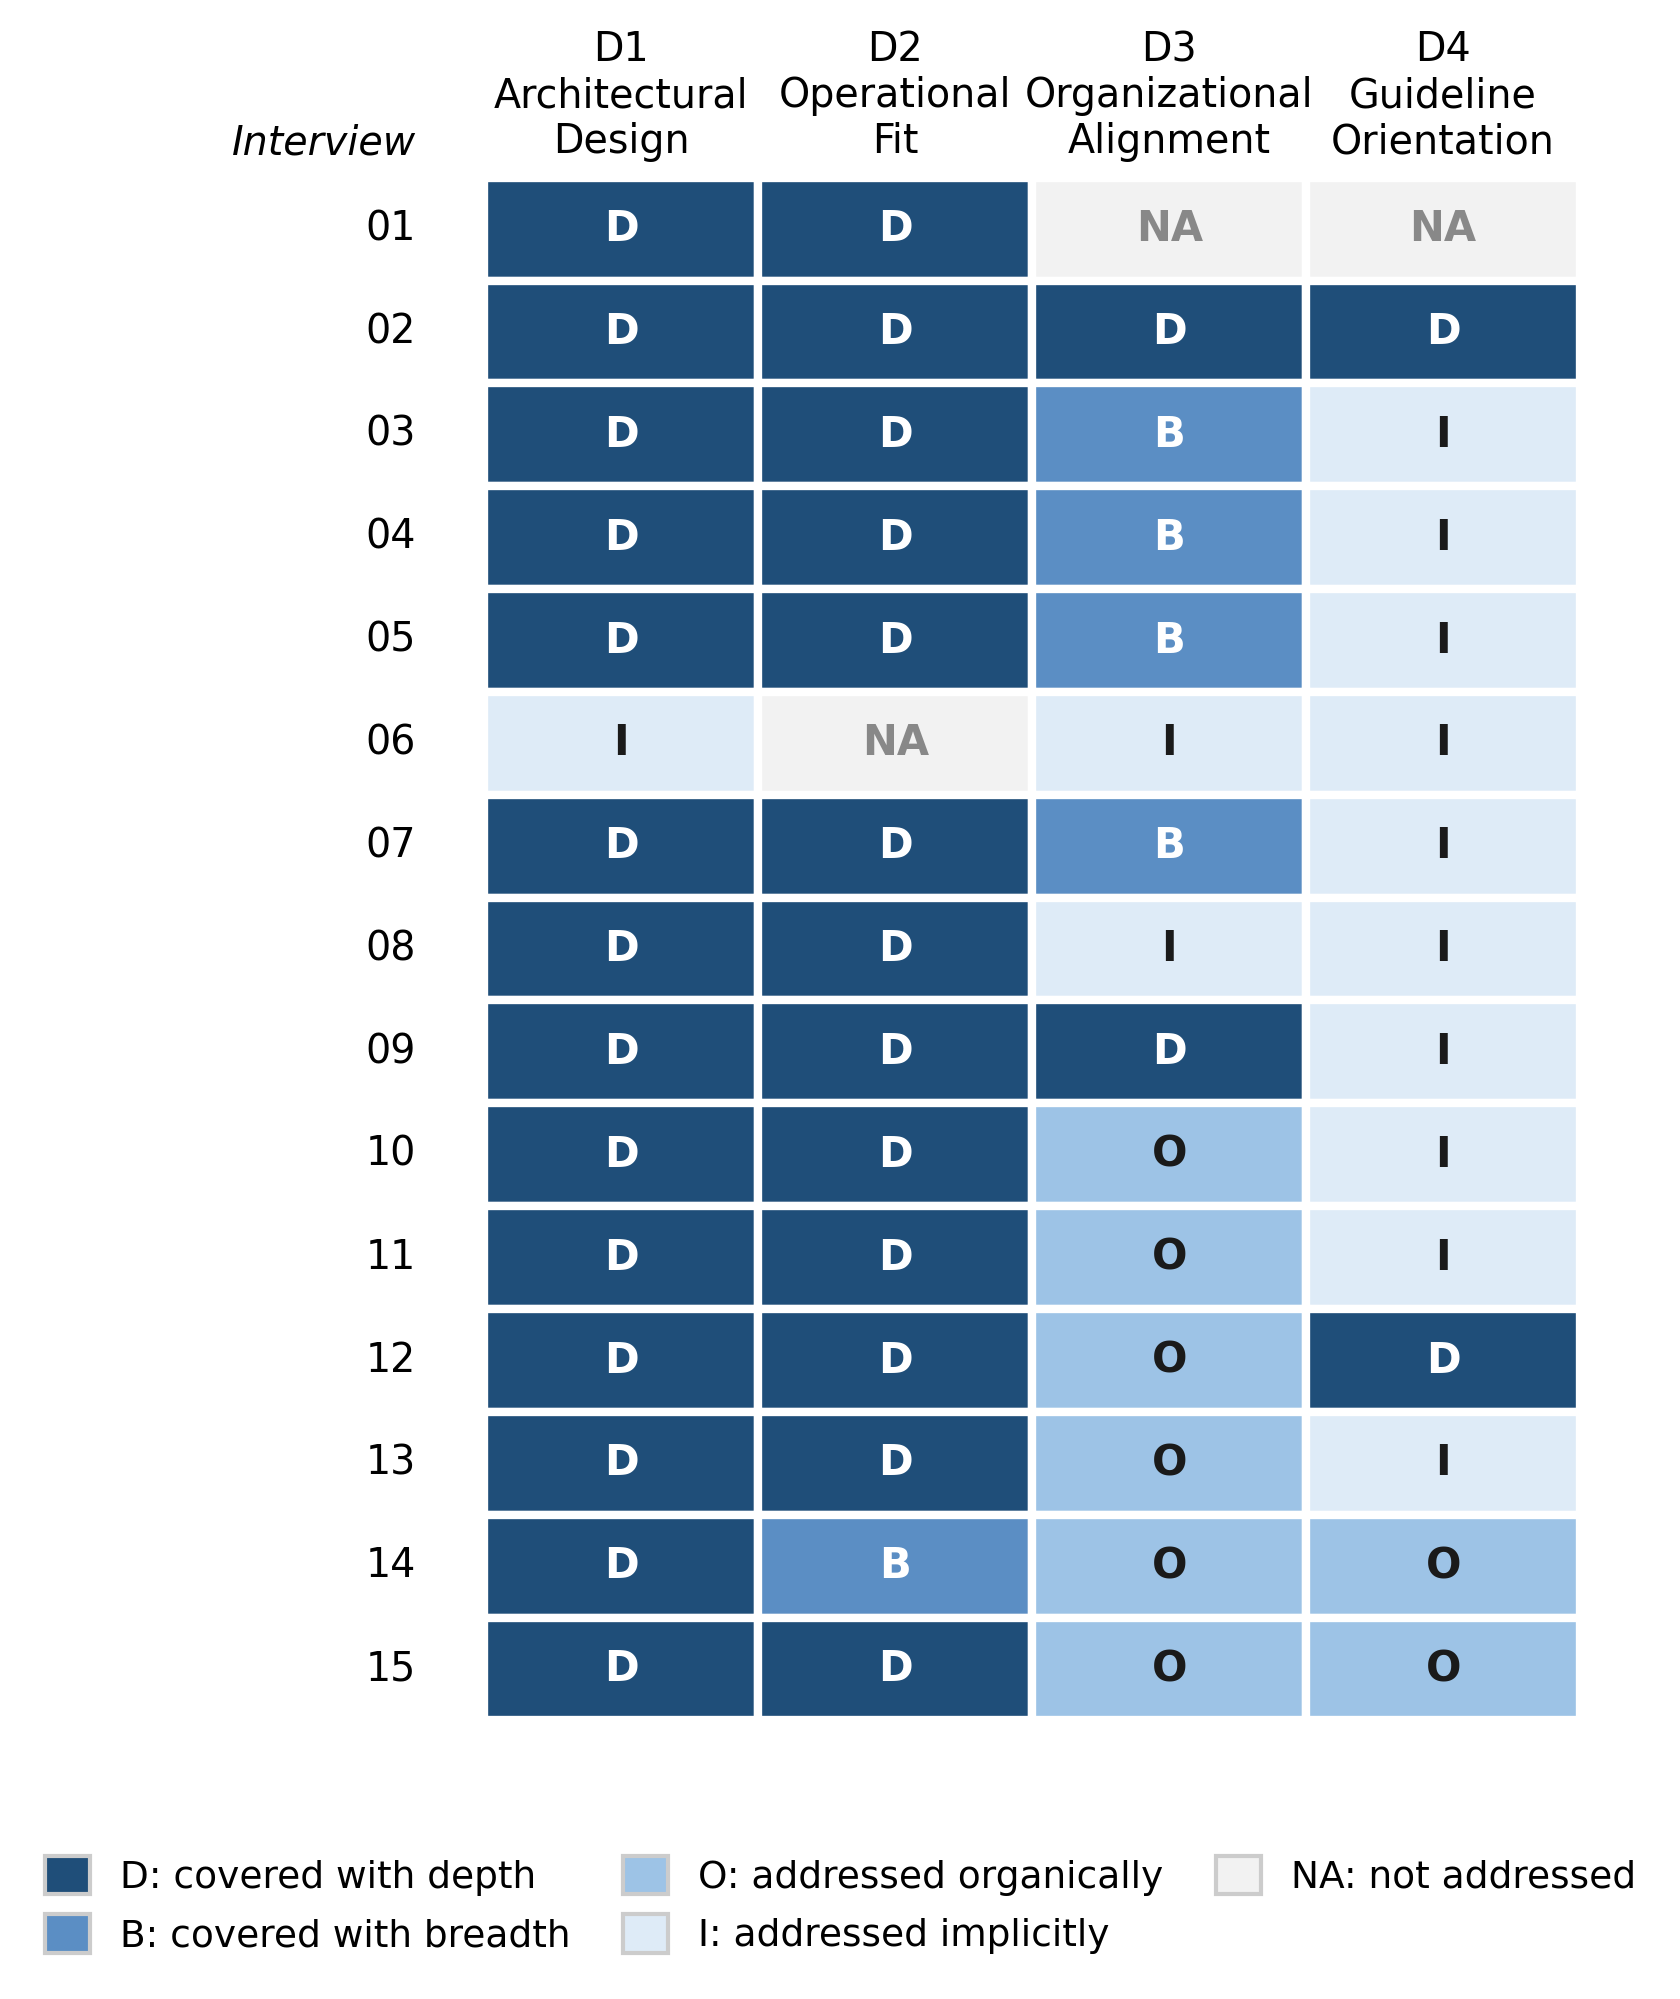
\includegraphics[width=0.78\textwidth]{ApeA/interviews_dimensions.png}
  \caption{Coverage of the four evaluation dimensions per session}
  \label{fig:interviews-dimensions}
\end{figure}

Two rows deserve comment:

\begin{enumerate}[itemsep=8pt,topsep=2pt]
  \item \emph{Interview 01.} The session used an earlier thirty-question script that produced the declared coverage gaps in D3 and D4; the protocol was revised to seven questions with one reserved for the deferred dimensions, and no subsequent session reproduced the gap.
  \item \emph{Interview 06.} The session focused on historical precedent and methodological advice rather than on probing the guidelines directly, which explains its lighter row.
\end{enumerate}

\subsection*{Saturation axes across the series}

Figure~\ref{fig:interviews-axes} consolidates the status of the five saturation axes tracked since Interview 01: A1 the spontaneous articulation of the Enforcement Gap, A2 the rigid-boundary and free-interior distinction, A3 pre-extraction sagas as actual practice, A4 observability as a systemic prerequisite, and A5 the reading of code listings as principle rather than prescription. The cells use four markers: \emph{R} for reaffirmed (fully or with a refinement), \emph{P} for partially reaffirmed (the substance was articulated without the named concept), \emph{C} for contested, and \emph{NA} for not addressed.

\begin{figure}[htb]
  \centering
  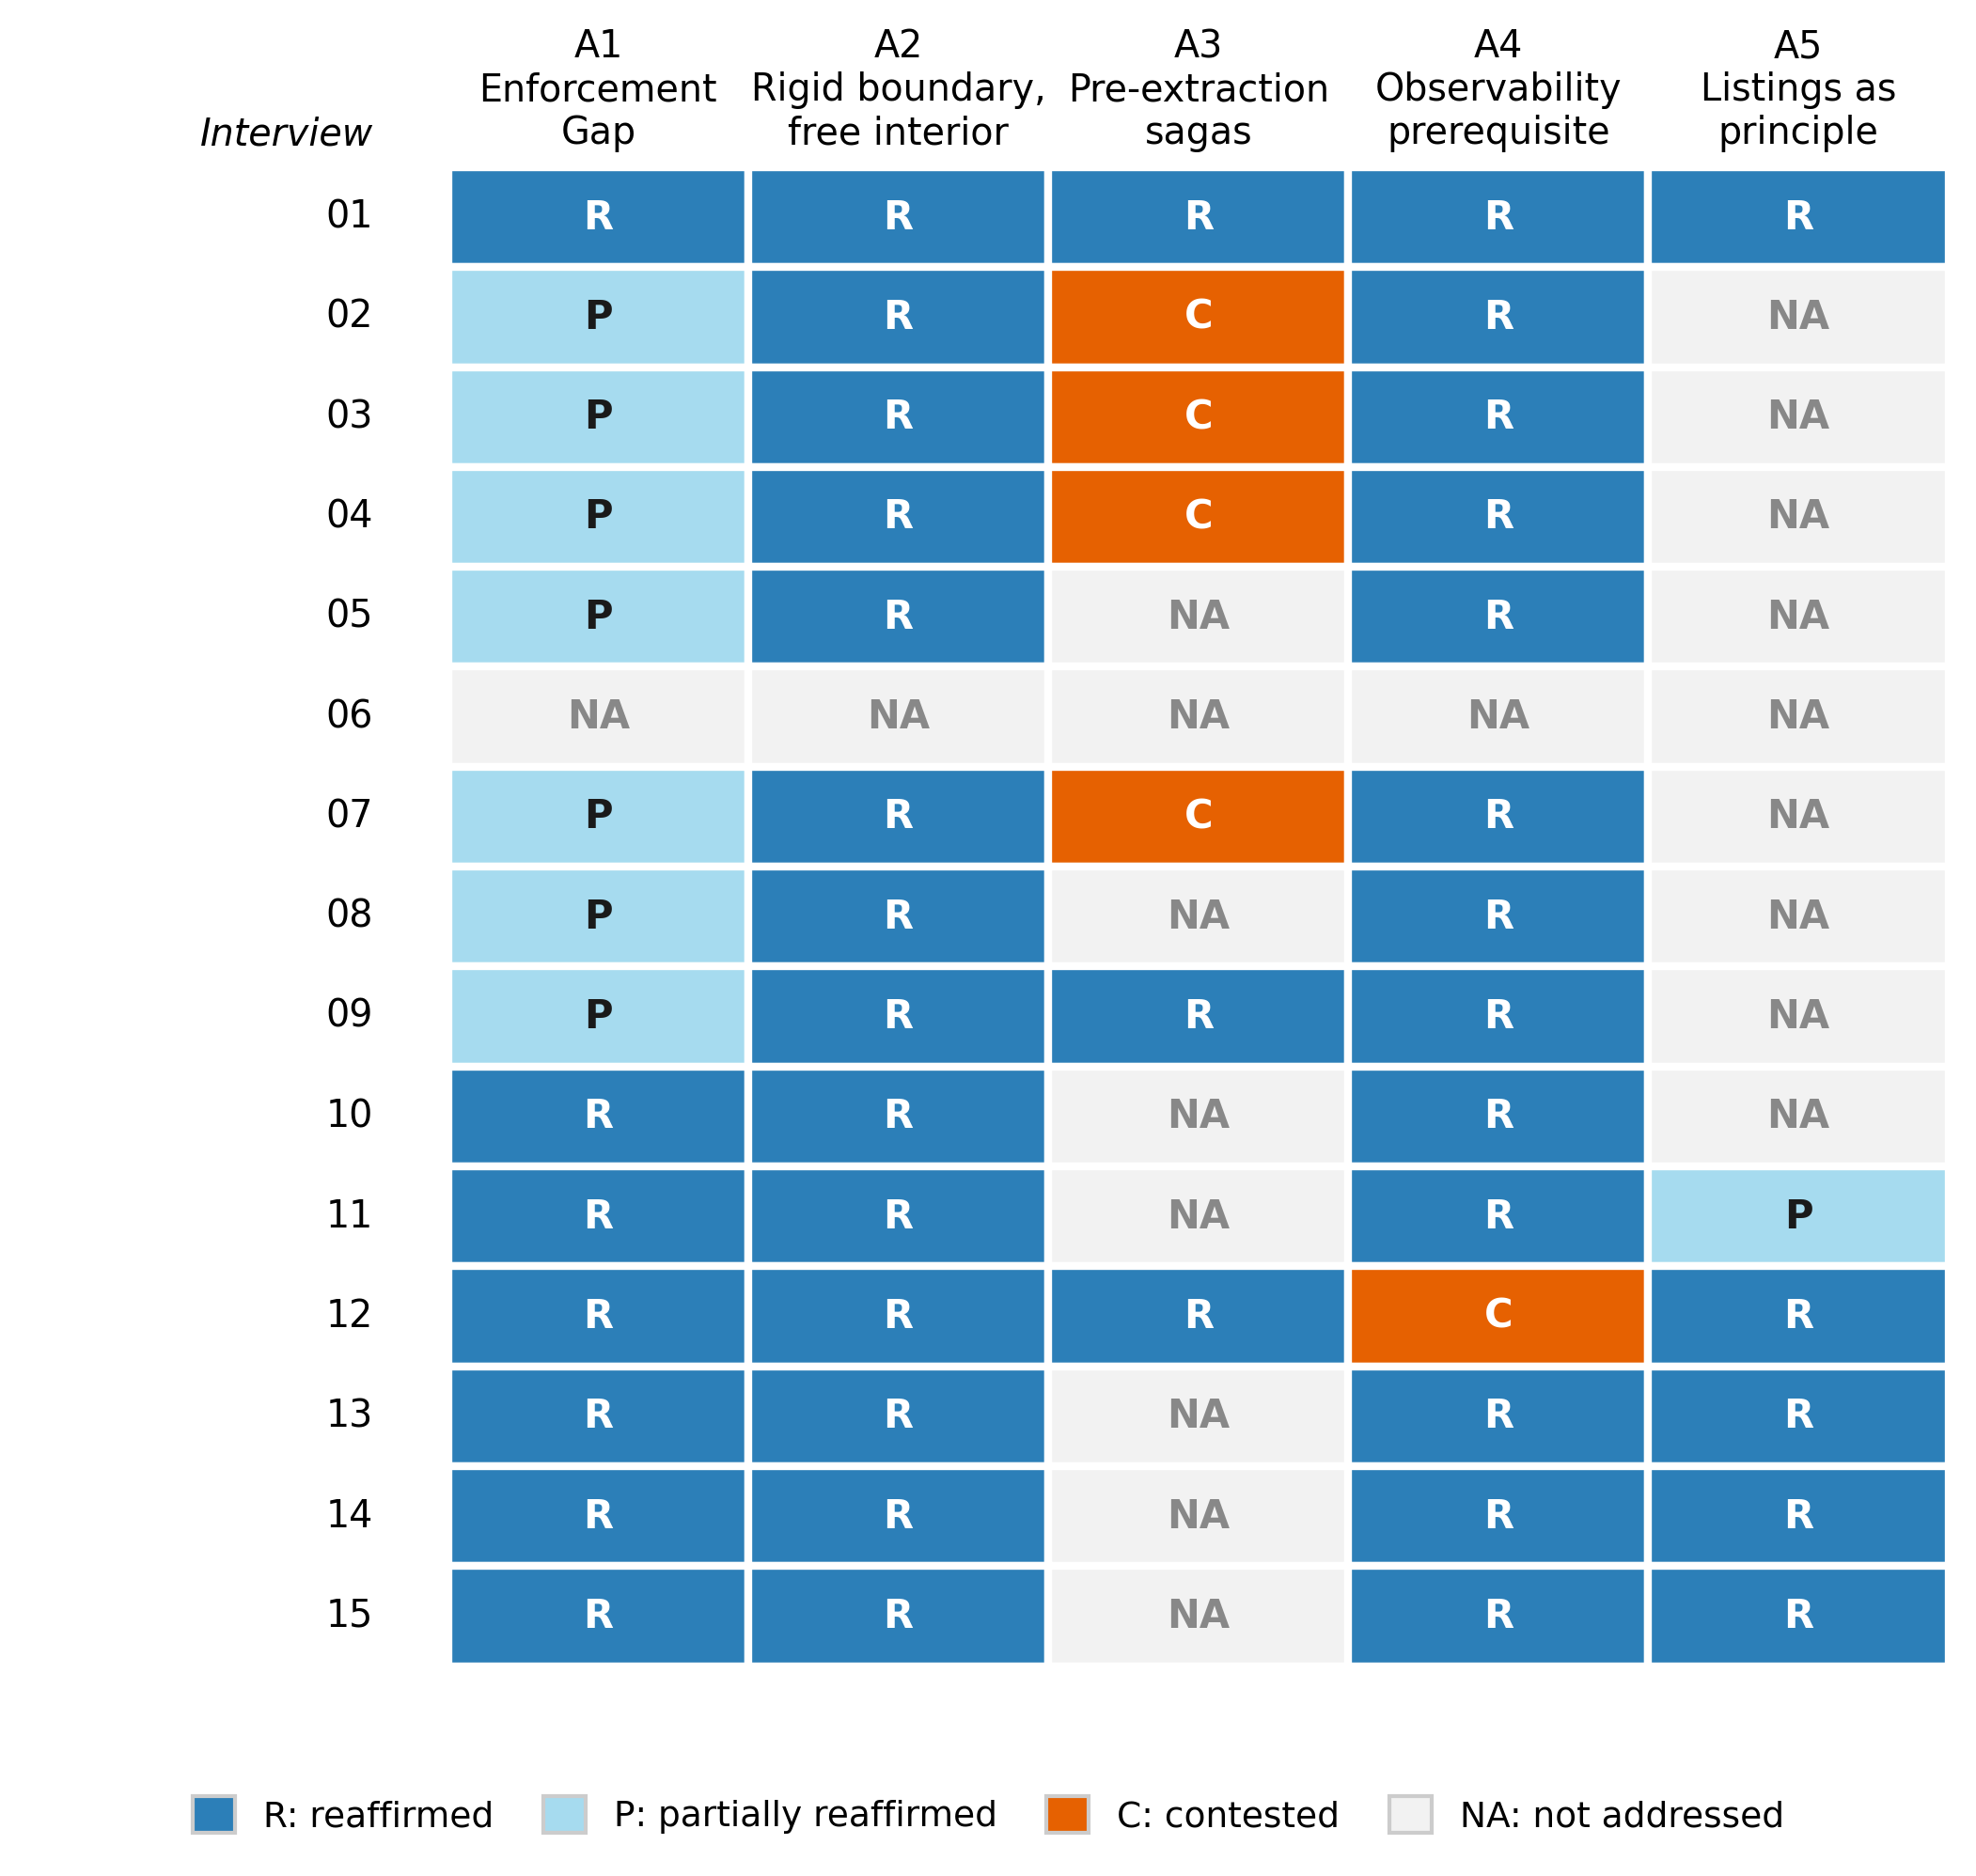
\includegraphics[width=0.88\textwidth]{ApeA/interviews_axes.png}
  \caption{Status of the five saturation axes per session}
  \label{fig:interviews-axes}
\end{figure}

Four rows deserve comment:

\begin{enumerate}[itemsep=8pt,topsep=2pt]
  \item \emph{Interview 01.} This is the session from which the five axes were declared, so its row records the original articulation rather than a reaffirmation.
  \item \emph{Interview 06.} The session did not probe the axes, consistent with its advisory character.
  \item \emph{Interview 09.} The session reaffirmed A3 by defending sagas as immediate value, against the contesting pattern of Interviews 02, 03, 04, and 07.
  \item \emph{Interview 12.} The session reaffirmed A3 conditional on a working saga boilerplate and contested A4 on timing grounds, arguing that the observability investment is premature for early-stage systems.
\end{enumerate}

The cross-series reading of the figure matches the synthesis reported in Chapter~\ref{sec:conclusion}:

\begin{enumerate}[itemsep=8pt,topsep=2pt]
  \item \emph{A1 Enforcement Gap.} The axis migrated from partial reaffirmations (substance without the term) in the early sessions to strong reaffirmations from Interview 10 onward.
  \item \emph{A2 Rigid boundary, free interior.} The axis was reaffirmed in every session that addressed it.
  \item \emph{A3 Pre-extraction sagas.} This is the only contested axis, with four contesting voices, two defending or conditional voices, and the remainder silent.
  \item \emph{A4 Observability prerequisite.} This is the most consolidated axis, reaffirmed in every session that addressed it except the timing-based contestation of Interview 12.
  \item \emph{A5 Listings as principle.} The axis was unaddressed by the early sessions and consistently reaffirmed from Interview 11 onward.
\end{enumerate}

The two-consecutive-sessions criterion declared in Appendix~\ref{ape:methodology} was not met during the series, so saturation is reported as a property of the series in the conclusions chapter, not claimed from any single session.
.
%% Consolidates the session metadata, interviewee attribution, dimension
%% coverage, and saturation-axis status of the fifteen interview reports.

\section{Series overview}
\label{sec:interviews-overview}

This chapter presents the fifteen expert interview reports of the verification phase. The methodology, the seven-question protocol, and the analysis framework are consolidated in Appendix~\ref{ape:methodology}. All sessions were remote synchronous video calls, recorded and transcribed, with verbal consent captured on record, and all were conducted in Brazilian Portuguese: quotations in the per-interview sections preserve the original wording, followed by an English translation for the reader.

This overview consolidates the descriptive information that is common to every report: session metadata (Table~\ref{tab:interviews-metadata}), interviewee attribution (Table~\ref{tab:interviews-attribution}), coverage of the four evaluation dimensions (Figure~\ref{fig:interviews-dimensions}), and the cross-series status of the five saturation axes (Figure~\ref{fig:interviews-axes}). The per-interview sections that follow keep the analytical content of each session: the three strongest themes, the verbatim quote worth preserving, the coded findings with their literature-gap mapping, the post-interview questionnaire findings, the session-specific limitations, the contributions to the conclusions chapter, and a concluding remark.

\subsection*{Session metadata}

Table~\ref{tab:interviews-metadata} records the date and the total recording length of each session.

\begin{longtable}{c l l}
\caption{Session metadata of the fifteen interviews.}
\label{tab:interviews-metadata}\\
\toprule
\textbf{Interview} & \textbf{Date (2026)} & \textbf{Recording} \\
\midrule
\endhead
\bottomrule
\endfoot
01 & 29 May & approx.\ 99 min \\
02 & 1 June & approx.\ 68 min \\
03 & 1 June & approx.\ 50 min \\
04 & 1 June & approx.\ 71 min \\
05 & 2 June & approx.\ 62 min \\
06 & 2 June & approx.\ 45 min \\
07 & 3 June & approx.\ 80 min \\
08 & 5 June & approx.\ 58 min \\
09 & 6 June & approx.\ 76 min \\
10 & 8 June & 56 min \\
11 & 8 June & 65 min \\
12 & 8 June & approx.\ 42 min \\
13 & 10 June & approx.\ 46 min \\
14 & 9 June & 37 min \\
15 & 9 June & approx.\ 29 min \\
\end{longtable}

Four sessions declared an analytical cutoff, the timestamp after which the conversation leaves research-relevant content; material after the cutoff does not appear in any derived artifact. The excluded segments are administrative or post-closing conversation:

\begin{enumerate}[itemsep=8pt,topsep=2pt]
  \item \emph{Interview 01, cutoff at 01:14:43.} A confirmation-letter discussion and employer-proprietary tool demos.
  \item \emph{Interview 02, cutoff at 01:07:25.} A product brainstorm derived from the maturity matrix discussion.
  \item \emph{Interview 03, cutoff at 00:49:40.} Defense logistics and prior-interview commentary.
  \item \emph{Interview 09, cutoff at 01:14:00.} Scheduling updates without analytical material.
\end{enumerate}

The remaining eleven sessions were research-relevant in full.

\subsection*{Interviewee attribution}

Table~\ref{tab:interviews-attribution} consolidates the attribution of the fifteen participants under the \emph{Interviewee N} scheme declared in Appendix~\ref{ape:methodology}. Personal identifiers are withheld in all cases, and the reports disclose the employment context at three levels: Interviews 01 to 07 name the industry but not the employer, Interviews 08, 10, 11, and 12 name previous employers and keep the current one undisclosed, and Interviews 09, 13, 14, and 15 withhold the organization entirely (the three public-sector participants work at a Brazilian state-owned information technology company, named only by category).

\begin{longtable}{c p{6.0cm} p{4.6cm} c}
\caption{Interviewee attribution across the series.}
\label{tab:interviews-attribution}\\
\toprule
\textbf{Interview} & \textbf{Role and context} & \textbf{Education} & \textbf{XP (yrs)} \\
\midrule
\endhead
\bottomrule
\endfoot
01 & Principal Software Engineer, U.S.\ telecommunications & BSc Information Technology & 16 \\
02 & Senior Engineering Manager, U.S.\ SaaS (home services) & Dipl\^ome d'Ing\'enieur, ENSIIE (France) & 15 \\
03 & CTO across Brazilian startups & BSc Information Technology & 14 \\
04 & Engineering Manager, Australian software company; former consultant & not declared & 15 \\
05 & Principal Software Engineer, Brazilian edtech & PhD student, Software Engineering & 17 \\
06 & Adjunct professor, federal Brazilian university & PhD Computer Science (2016) & n/d \\
07 & Engineering Manager, Brazilian fintech & BSc Information Systems & 12 \\
08 & Principal Software Engineer, formerly at Shopify & Engineering degree & 10+ \\
09 & Software engineer, distributed and modular monolith systems & Dipl\^ome d'Ing\'enieur, \'Ecole Polytechnique; BEng Poli-USP & 4 \\
10 & Senior Software Engineer, formerly at GitHub and Red Hat & Engineering degree & 14 to 15 \\
11 & Software engineer, formerly at Samsung SRBR, Ita\'u, Viva Real & MSc Computer Science, UFAM & 10+ \\
12 & Backend Software Engineer, formerly at VR Benef\'icios and Ambev & Technologist, Systems Analysis, IFSP & 7 \\
13 & Engineering Manager, state-owned IT company (public sector) & MSc UFMG; doctoral student & 13 \\
14 & Software Engineer, state-owned IT company (public sector) & BSc Computer Science, UniBH & 10 \\
15 & Systems Analyst, state-owned IT company (public sector) & Technologist, Systems Analysis, Una & 13 \\
\end{longtable}

The profile categories tracked across the series are eleven industry practitioners, three mixed industry-and-academic profiles (Interviews 05, 11, and 13), and one academic researcher (Interview 06). The sample covers Brazilian, Australian, French, and United States contexts, with years of professional experience from four to seventeen.

\subsection*{Coverage of the four evaluation dimensions}

Figure~\ref{fig:interviews-dimensions} shows how thoroughly each session covered the four evaluation dimensions: D1 Architectural Design, D2 Operational Fit, D3 Organizational Alignment, and D4 Guideline Orientation. The cells use five markers: \emph{D} for covered with depth, \emph{B} for covered with breadth or covered more briefly, \emph{O} for addressed organically (the participant raised the dimension without prompting), \emph{I} for addressed implicitly or indirectly, and \emph{NA} for not addressed.

\begin{figure}[htb]
  \centering
  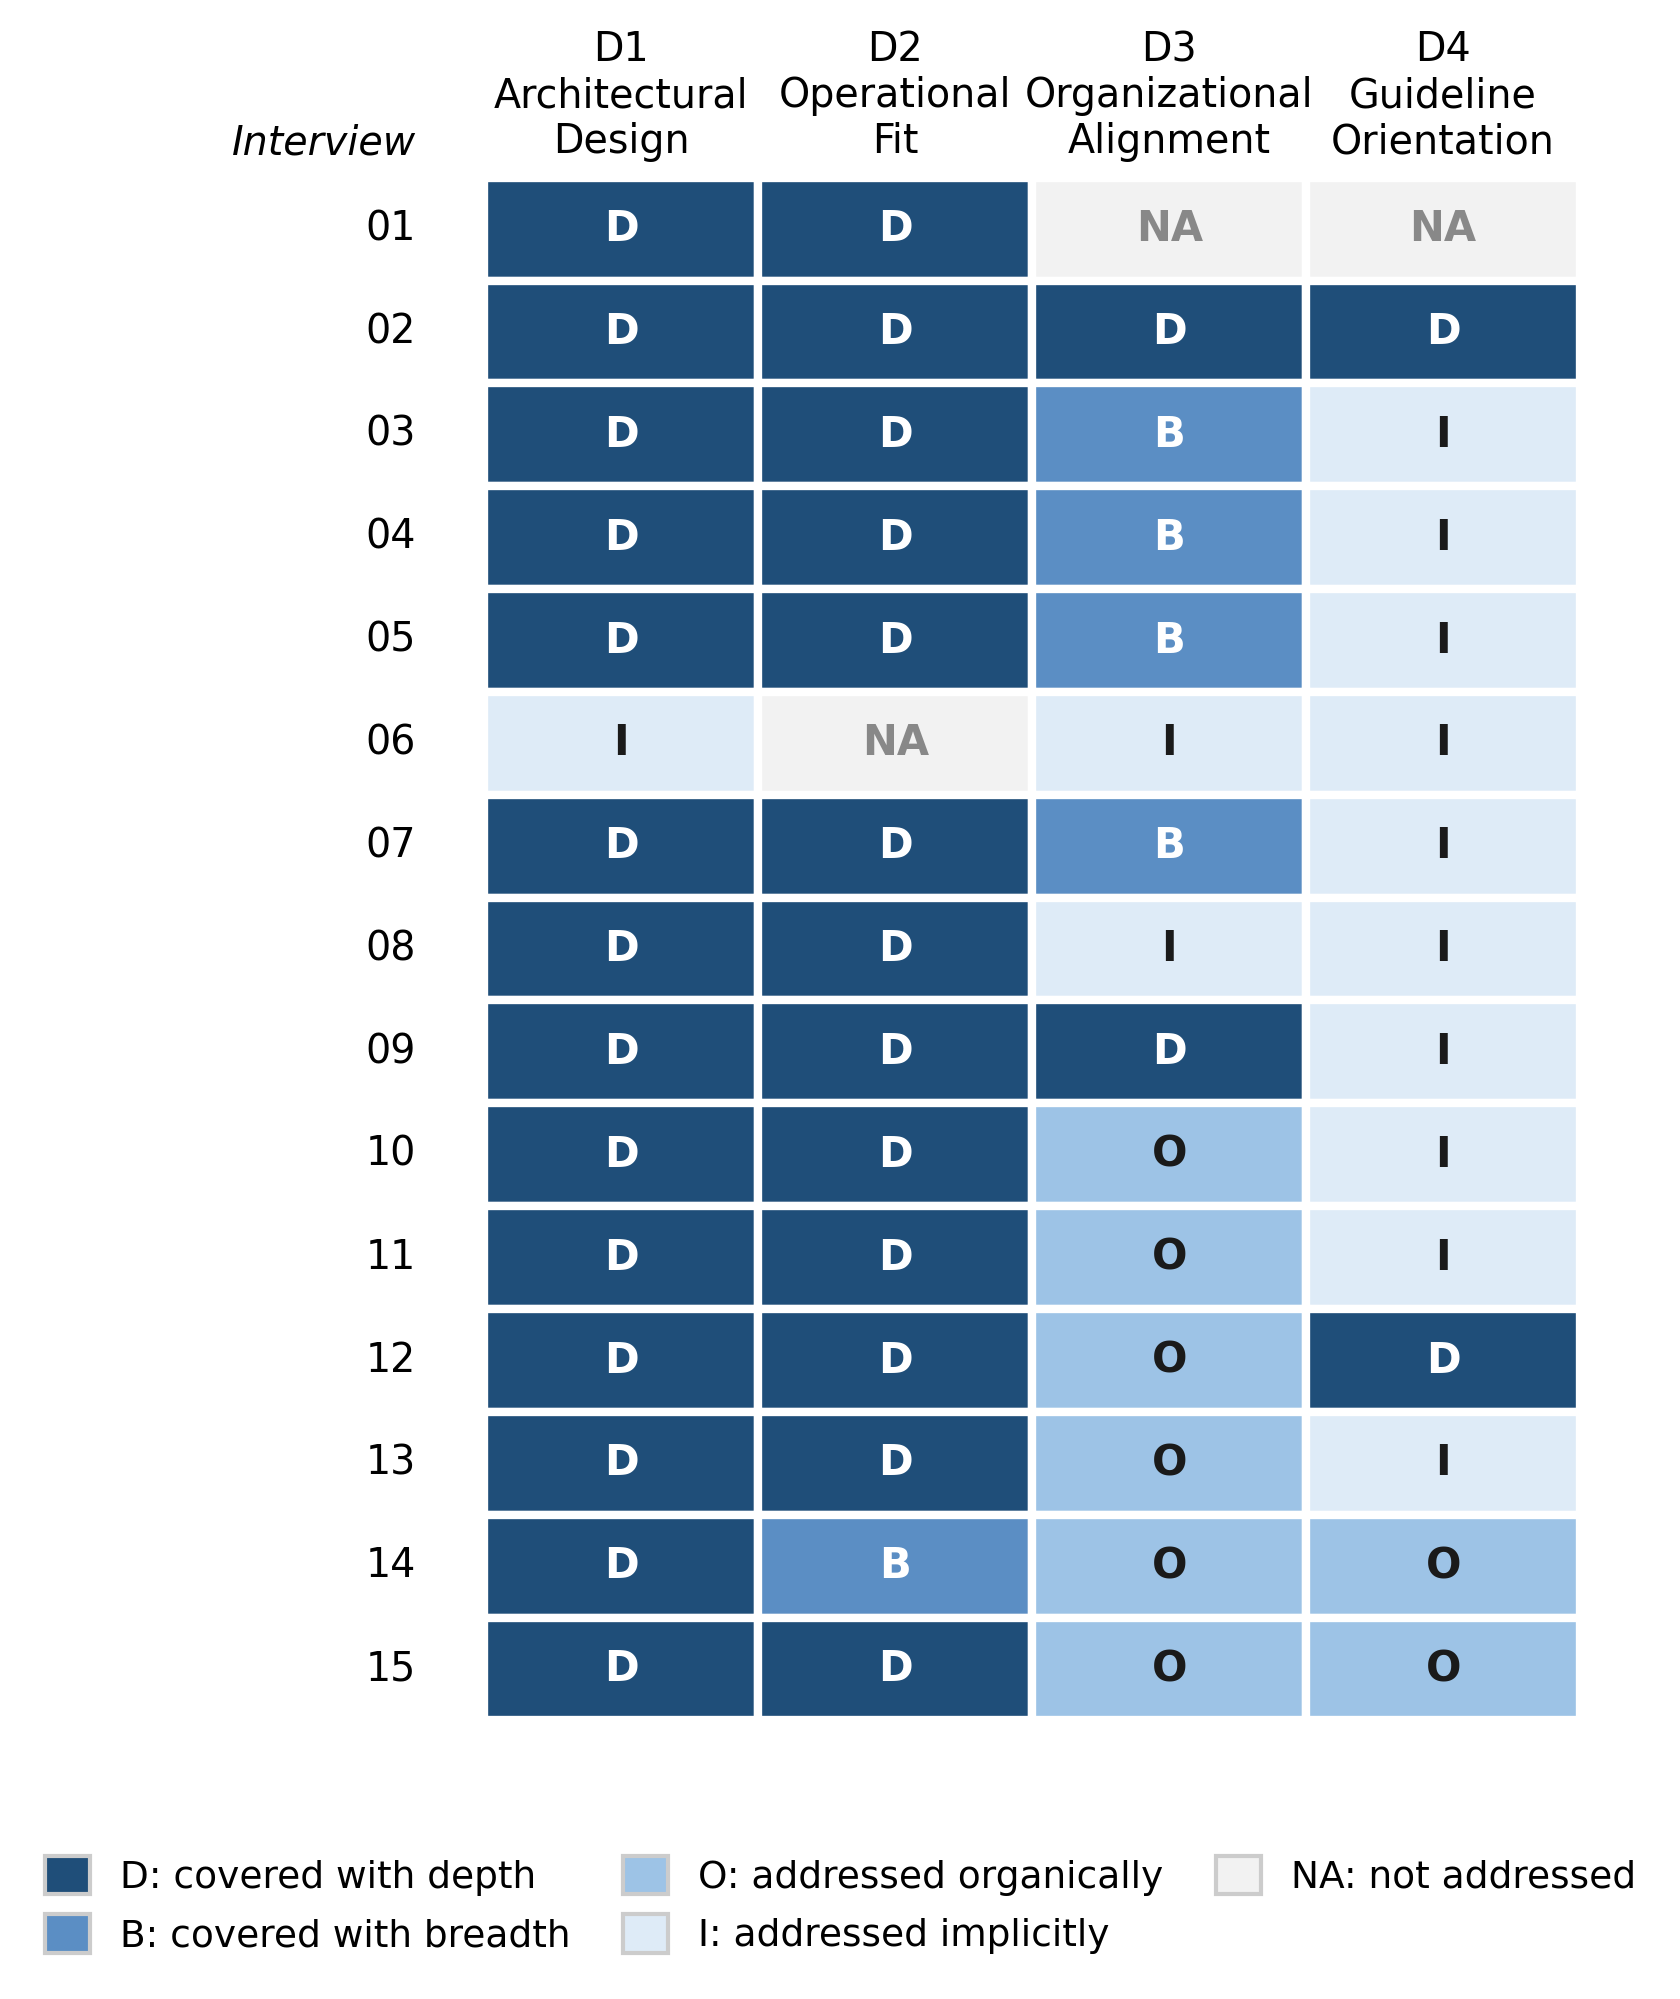
\includegraphics[width=0.78\textwidth]{ApeA/interviews_dimensions.png}
  \caption{Coverage of the four evaluation dimensions per session}
  \label{fig:interviews-dimensions}
\end{figure}

Two rows deserve comment:

\begin{enumerate}[itemsep=8pt,topsep=2pt]
  \item \emph{Interview 01.} The session used an earlier thirty-question script that produced the declared coverage gaps in D3 and D4; the protocol was revised to seven questions with one reserved for the deferred dimensions, and no subsequent session reproduced the gap.
  \item \emph{Interview 06.} The session focused on historical precedent and methodological advice rather than on probing the guidelines directly, which explains its lighter row.
\end{enumerate}

\subsection*{Saturation axes across the series}

Figure~\ref{fig:interviews-axes} consolidates the status of the five saturation axes tracked since Interview 01: A1 the spontaneous articulation of the Enforcement Gap, A2 the rigid-boundary and free-interior distinction, A3 pre-extraction sagas as actual practice, A4 observability as a systemic prerequisite, and A5 the reading of code listings as principle rather than prescription. The cells use four markers: \emph{R} for reaffirmed (fully or with a refinement), \emph{P} for partially reaffirmed (the substance was articulated without the named concept), \emph{C} for contested, and \emph{NA} for not addressed.

\begin{figure}[htb]
  \centering
  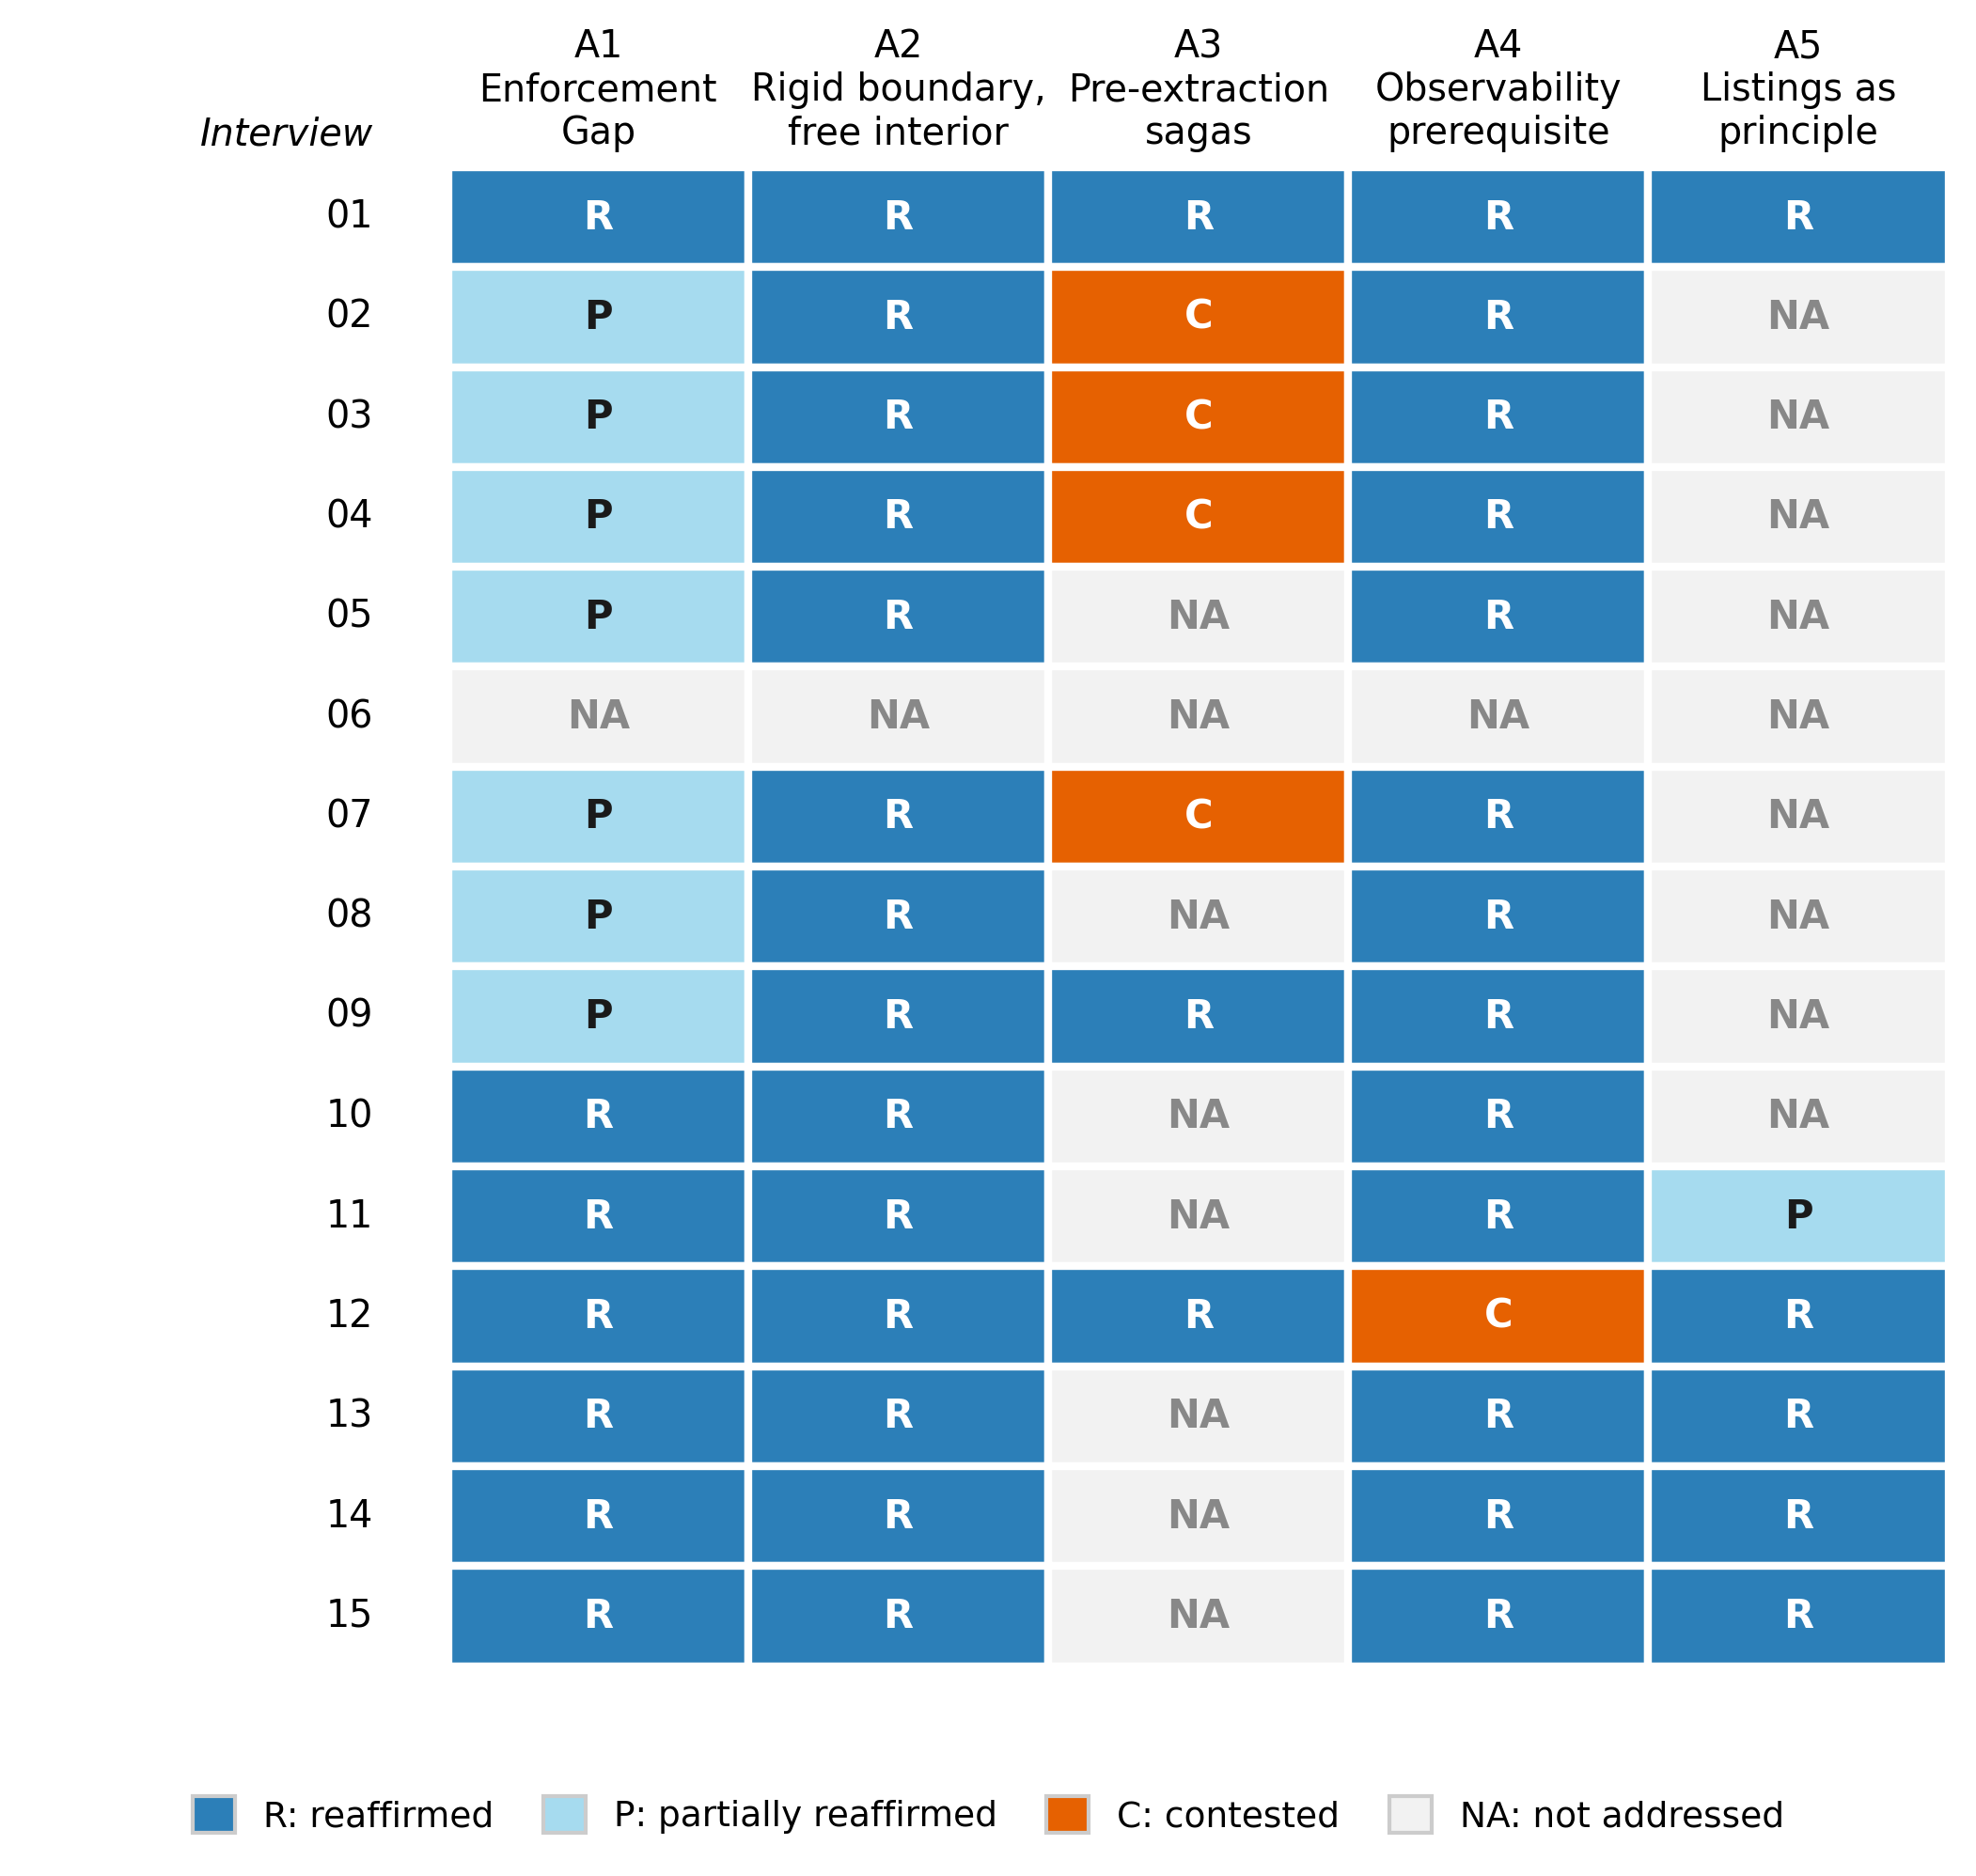
\includegraphics[width=0.88\textwidth]{ApeA/interviews_axes.png}
  \caption{Status of the five saturation axes per session}
  \label{fig:interviews-axes}
\end{figure}

Four rows deserve comment:

\begin{enumerate}[itemsep=8pt,topsep=2pt]
  \item \emph{Interview 01.} This is the session from which the five axes were declared, so its row records the original articulation rather than a reaffirmation.
  \item \emph{Interview 06.} The session did not probe the axes, consistent with its advisory character.
  \item \emph{Interview 09.} The session reaffirmed A3 by defending sagas as immediate value, against the contesting pattern of Interviews 02, 03, 04, and 07.
  \item \emph{Interview 12.} The session reaffirmed A3 conditional on a working saga boilerplate and contested A4 on timing grounds, arguing that the observability investment is premature for early-stage systems.
\end{enumerate}

The cross-series reading of the figure matches the synthesis reported in Chapter~\ref{sec:conclusion}:

\begin{enumerate}[itemsep=8pt,topsep=2pt]
  \item \emph{A1 Enforcement Gap.} The axis migrated from partial reaffirmations (substance without the term) in the early sessions to strong reaffirmations from Interview 10 onward.
  \item \emph{A2 Rigid boundary, free interior.} The axis was reaffirmed in every session that addressed it.
  \item \emph{A3 Pre-extraction sagas.} This is the only contested axis, with four contesting voices, two defending or conditional voices, and the remainder silent.
  \item \emph{A4 Observability prerequisite.} This is the most consolidated axis, reaffirmed in every session that addressed it except the timing-based contestation of Interview 12.
  \item \emph{A5 Listings as principle.} The axis was unaddressed by the early sessions and consistently reaffirmed from Interview 11 onward.
\end{enumerate}

The two-consecutive-sessions criterion declared in Appendix~\ref{ape:methodology} was not met during the series, so saturation is reported as a property of the series in the conclusions chapter, not claimed from any single session.
.
%% Consolidates the session metadata, interviewee attribution, dimension
%% coverage, and saturation-axis status of the fifteen interview reports.

\section{Series overview}
\label{sec:interviews-overview}

This chapter presents the fifteen expert interview reports of the verification phase. The methodology, the seven-question protocol, and the analysis framework are consolidated in Appendix~\ref{ape:methodology}. All sessions were remote synchronous video calls, recorded and transcribed, with verbal consent captured on record, and all were conducted in Brazilian Portuguese: quotations in the per-interview sections preserve the original wording, followed by an English translation for the reader.

This overview consolidates the descriptive information that is common to every report: session metadata (Table~\ref{tab:interviews-metadata}), interviewee attribution (Table~\ref{tab:interviews-attribution}), coverage of the four evaluation dimensions (Figure~\ref{fig:interviews-dimensions}), and the cross-series status of the five saturation axes (Figure~\ref{fig:interviews-axes}). The per-interview sections that follow keep the analytical content of each session: the three strongest themes, the verbatim quote worth preserving, the coded findings with their literature-gap mapping, the post-interview questionnaire findings, the session-specific limitations, the contributions to the conclusions chapter, and a concluding remark.

\subsection*{Session metadata}

Table~\ref{tab:interviews-metadata} records the date and the total recording length of each session.

\begin{longtable}{c l l}
\caption{Session metadata of the fifteen interviews.}
\label{tab:interviews-metadata}\\
\toprule
\textbf{Interview} & \textbf{Date (2026)} & \textbf{Recording} \\
\midrule
\endhead
\bottomrule
\endfoot
01 & 29 May & approx.\ 99 min \\
02 & 1 June & approx.\ 68 min \\
03 & 1 June & approx.\ 50 min \\
04 & 1 June & approx.\ 71 min \\
05 & 2 June & approx.\ 62 min \\
06 & 2 June & approx.\ 45 min \\
07 & 3 June & approx.\ 80 min \\
08 & 5 June & approx.\ 58 min \\
09 & 6 June & approx.\ 76 min \\
10 & 8 June & 56 min \\
11 & 8 June & 65 min \\
12 & 8 June & approx.\ 42 min \\
13 & 10 June & approx.\ 46 min \\
14 & 9 June & 37 min \\
15 & 9 June & approx.\ 29 min \\
\end{longtable}

Four sessions declared an analytical cutoff, the timestamp after which the conversation leaves research-relevant content; material after the cutoff does not appear in any derived artifact. The excluded segments are administrative or post-closing conversation:

\begin{enumerate}[itemsep=8pt,topsep=2pt]
  \item \emph{Interview 01, cutoff at 01:14:43.} A confirmation-letter discussion and employer-proprietary tool demos.
  \item \emph{Interview 02, cutoff at 01:07:25.} A product brainstorm derived from the maturity matrix discussion.
  \item \emph{Interview 03, cutoff at 00:49:40.} Defense logistics and prior-interview commentary.
  \item \emph{Interview 09, cutoff at 01:14:00.} Scheduling updates without analytical material.
\end{enumerate}

The remaining eleven sessions were research-relevant in full.

\subsection*{Interviewee attribution}

Table~\ref{tab:interviews-attribution} consolidates the attribution of the fifteen participants under the \emph{Interviewee N} scheme declared in Appendix~\ref{ape:methodology}. Personal identifiers are withheld in all cases, and the reports disclose the employment context at three levels: Interviews 01 to 07 name the industry but not the employer, Interviews 08, 10, 11, and 12 name previous employers and keep the current one undisclosed, and Interviews 09, 13, 14, and 15 withhold the organization entirely (the three public-sector participants work at a Brazilian state-owned information technology company, named only by category).

\begin{longtable}{c p{6.0cm} p{4.6cm} c}
\caption{Interviewee attribution across the series.}
\label{tab:interviews-attribution}\\
\toprule
\textbf{Interview} & \textbf{Role and context} & \textbf{Education} & \textbf{XP (yrs)} \\
\midrule
\endhead
\bottomrule
\endfoot
01 & Principal Software Engineer, U.S.\ telecommunications & BSc Information Technology & 16 \\
02 & Senior Engineering Manager, U.S.\ SaaS (home services) & Dipl\^ome d'Ing\'enieur, ENSIIE (France) & 15 \\
03 & CTO across Brazilian startups & BSc Information Technology & 14 \\
04 & Engineering Manager, Australian software company; former consultant & not declared & 15 \\
05 & Principal Software Engineer, Brazilian edtech & PhD student, Software Engineering & 17 \\
06 & Adjunct professor, federal Brazilian university & PhD Computer Science (2016) & n/d \\
07 & Engineering Manager, Brazilian fintech & BSc Information Systems & 12 \\
08 & Principal Software Engineer, formerly at Shopify & Engineering degree & 10+ \\
09 & Software engineer, distributed and modular monolith systems & Dipl\^ome d'Ing\'enieur, \'Ecole Polytechnique; BEng Poli-USP & 4 \\
10 & Senior Software Engineer, formerly at GitHub and Red Hat & Engineering degree & 14 to 15 \\
11 & Software engineer, formerly at Samsung SRBR, Ita\'u, Viva Real & MSc Computer Science, UFAM & 10+ \\
12 & Backend Software Engineer, formerly at VR Benef\'icios and Ambev & Technologist, Systems Analysis, IFSP & 7 \\
13 & Engineering Manager, state-owned IT company (public sector) & MSc UFMG; doctoral student & 13 \\
14 & Software Engineer, state-owned IT company (public sector) & BSc Computer Science, UniBH & 10 \\
15 & Systems Analyst, state-owned IT company (public sector) & Technologist, Systems Analysis, Una & 13 \\
\end{longtable}

The profile categories tracked across the series are eleven industry practitioners, three mixed industry-and-academic profiles (Interviews 05, 11, and 13), and one academic researcher (Interview 06). The sample covers Brazilian, Australian, French, and United States contexts, with years of professional experience from four to seventeen.

\subsection*{Coverage of the four evaluation dimensions}

Figure~\ref{fig:interviews-dimensions} shows how thoroughly each session covered the four evaluation dimensions: D1 Architectural Design, D2 Operational Fit, D3 Organizational Alignment, and D4 Guideline Orientation. The cells use five markers: \emph{D} for covered with depth, \emph{B} for covered with breadth or covered more briefly, \emph{O} for addressed organically (the participant raised the dimension without prompting), \emph{I} for addressed implicitly or indirectly, and \emph{NA} for not addressed.

\begin{figure}[htb]
  \centering
  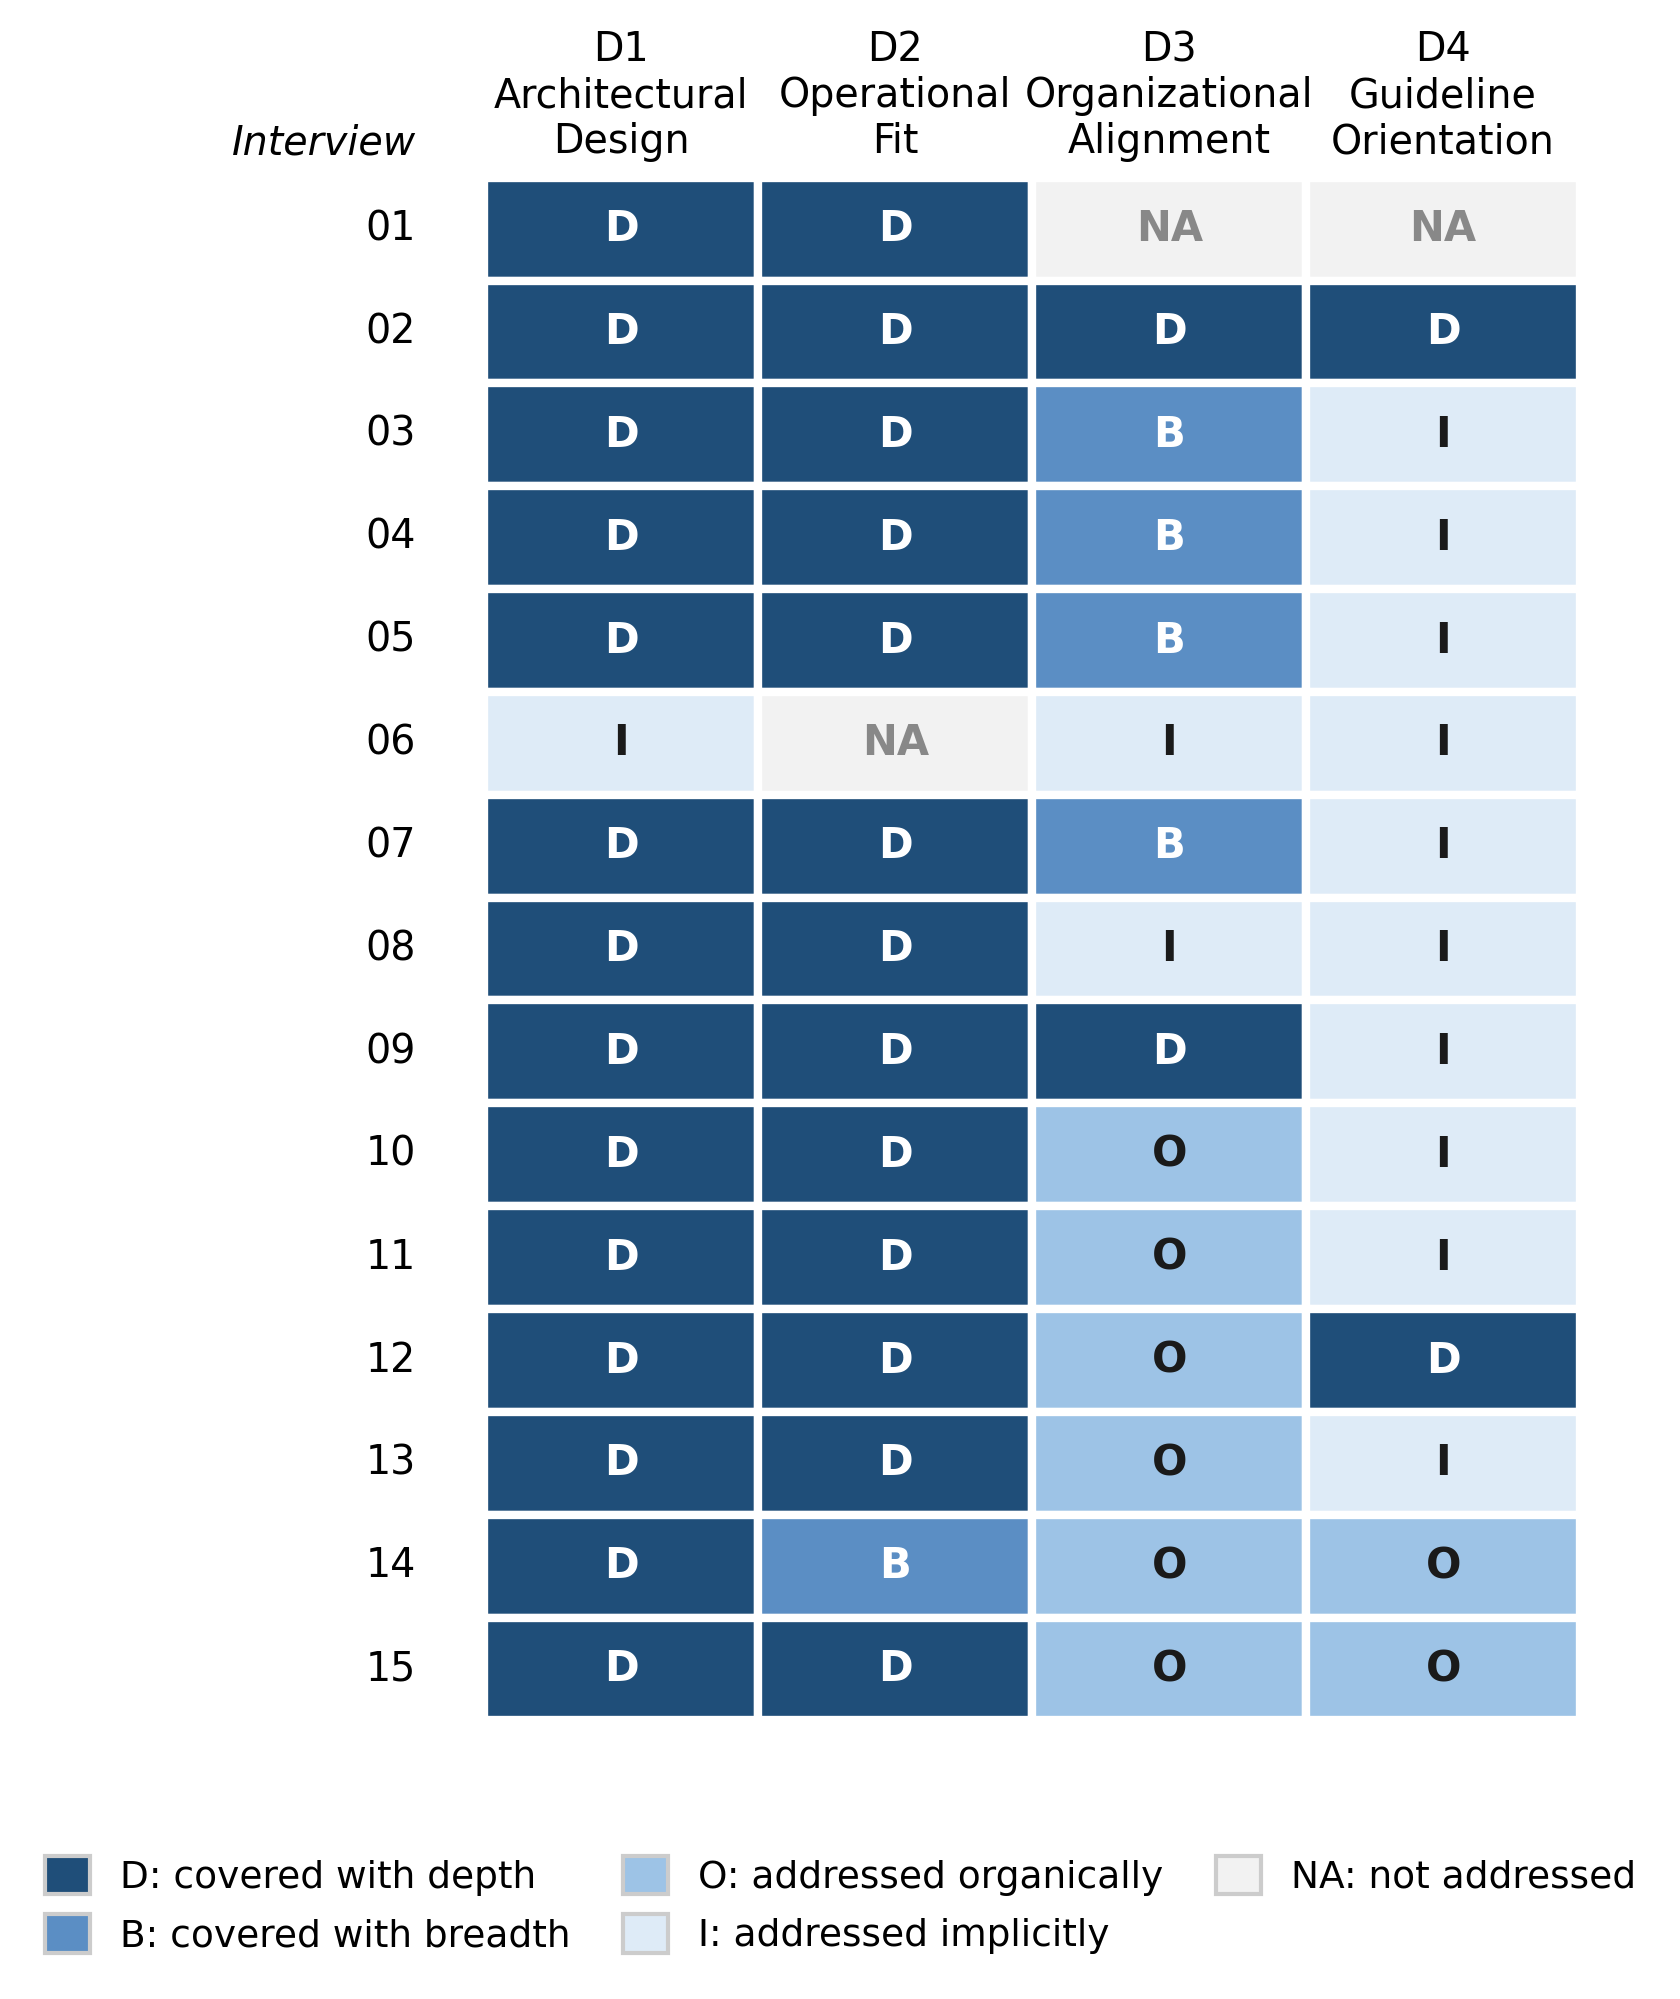
\includegraphics[width=0.78\textwidth]{ApeA/interviews_dimensions.png}
  \caption{Coverage of the four evaluation dimensions per session}
  \label{fig:interviews-dimensions}
\end{figure}

Two rows deserve comment:

\begin{enumerate}[itemsep=8pt,topsep=2pt]
  \item \emph{Interview 01.} The session used an earlier thirty-question script that produced the declared coverage gaps in D3 and D4; the protocol was revised to seven questions with one reserved for the deferred dimensions, and no subsequent session reproduced the gap.
  \item \emph{Interview 06.} The session focused on historical precedent and methodological advice rather than on probing the guidelines directly, which explains its lighter row.
\end{enumerate}

\subsection*{Saturation axes across the series}

Figure~\ref{fig:interviews-axes} consolidates the status of the five saturation axes tracked since Interview 01: A1 the spontaneous articulation of the Enforcement Gap, A2 the rigid-boundary and free-interior distinction, A3 pre-extraction sagas as actual practice, A4 observability as a systemic prerequisite, and A5 the reading of code listings as principle rather than prescription. The cells use four markers: \emph{R} for reaffirmed (fully or with a refinement), \emph{P} for partially reaffirmed (the substance was articulated without the named concept), \emph{C} for contested, and \emph{NA} for not addressed.

\begin{figure}[htb]
  \centering
  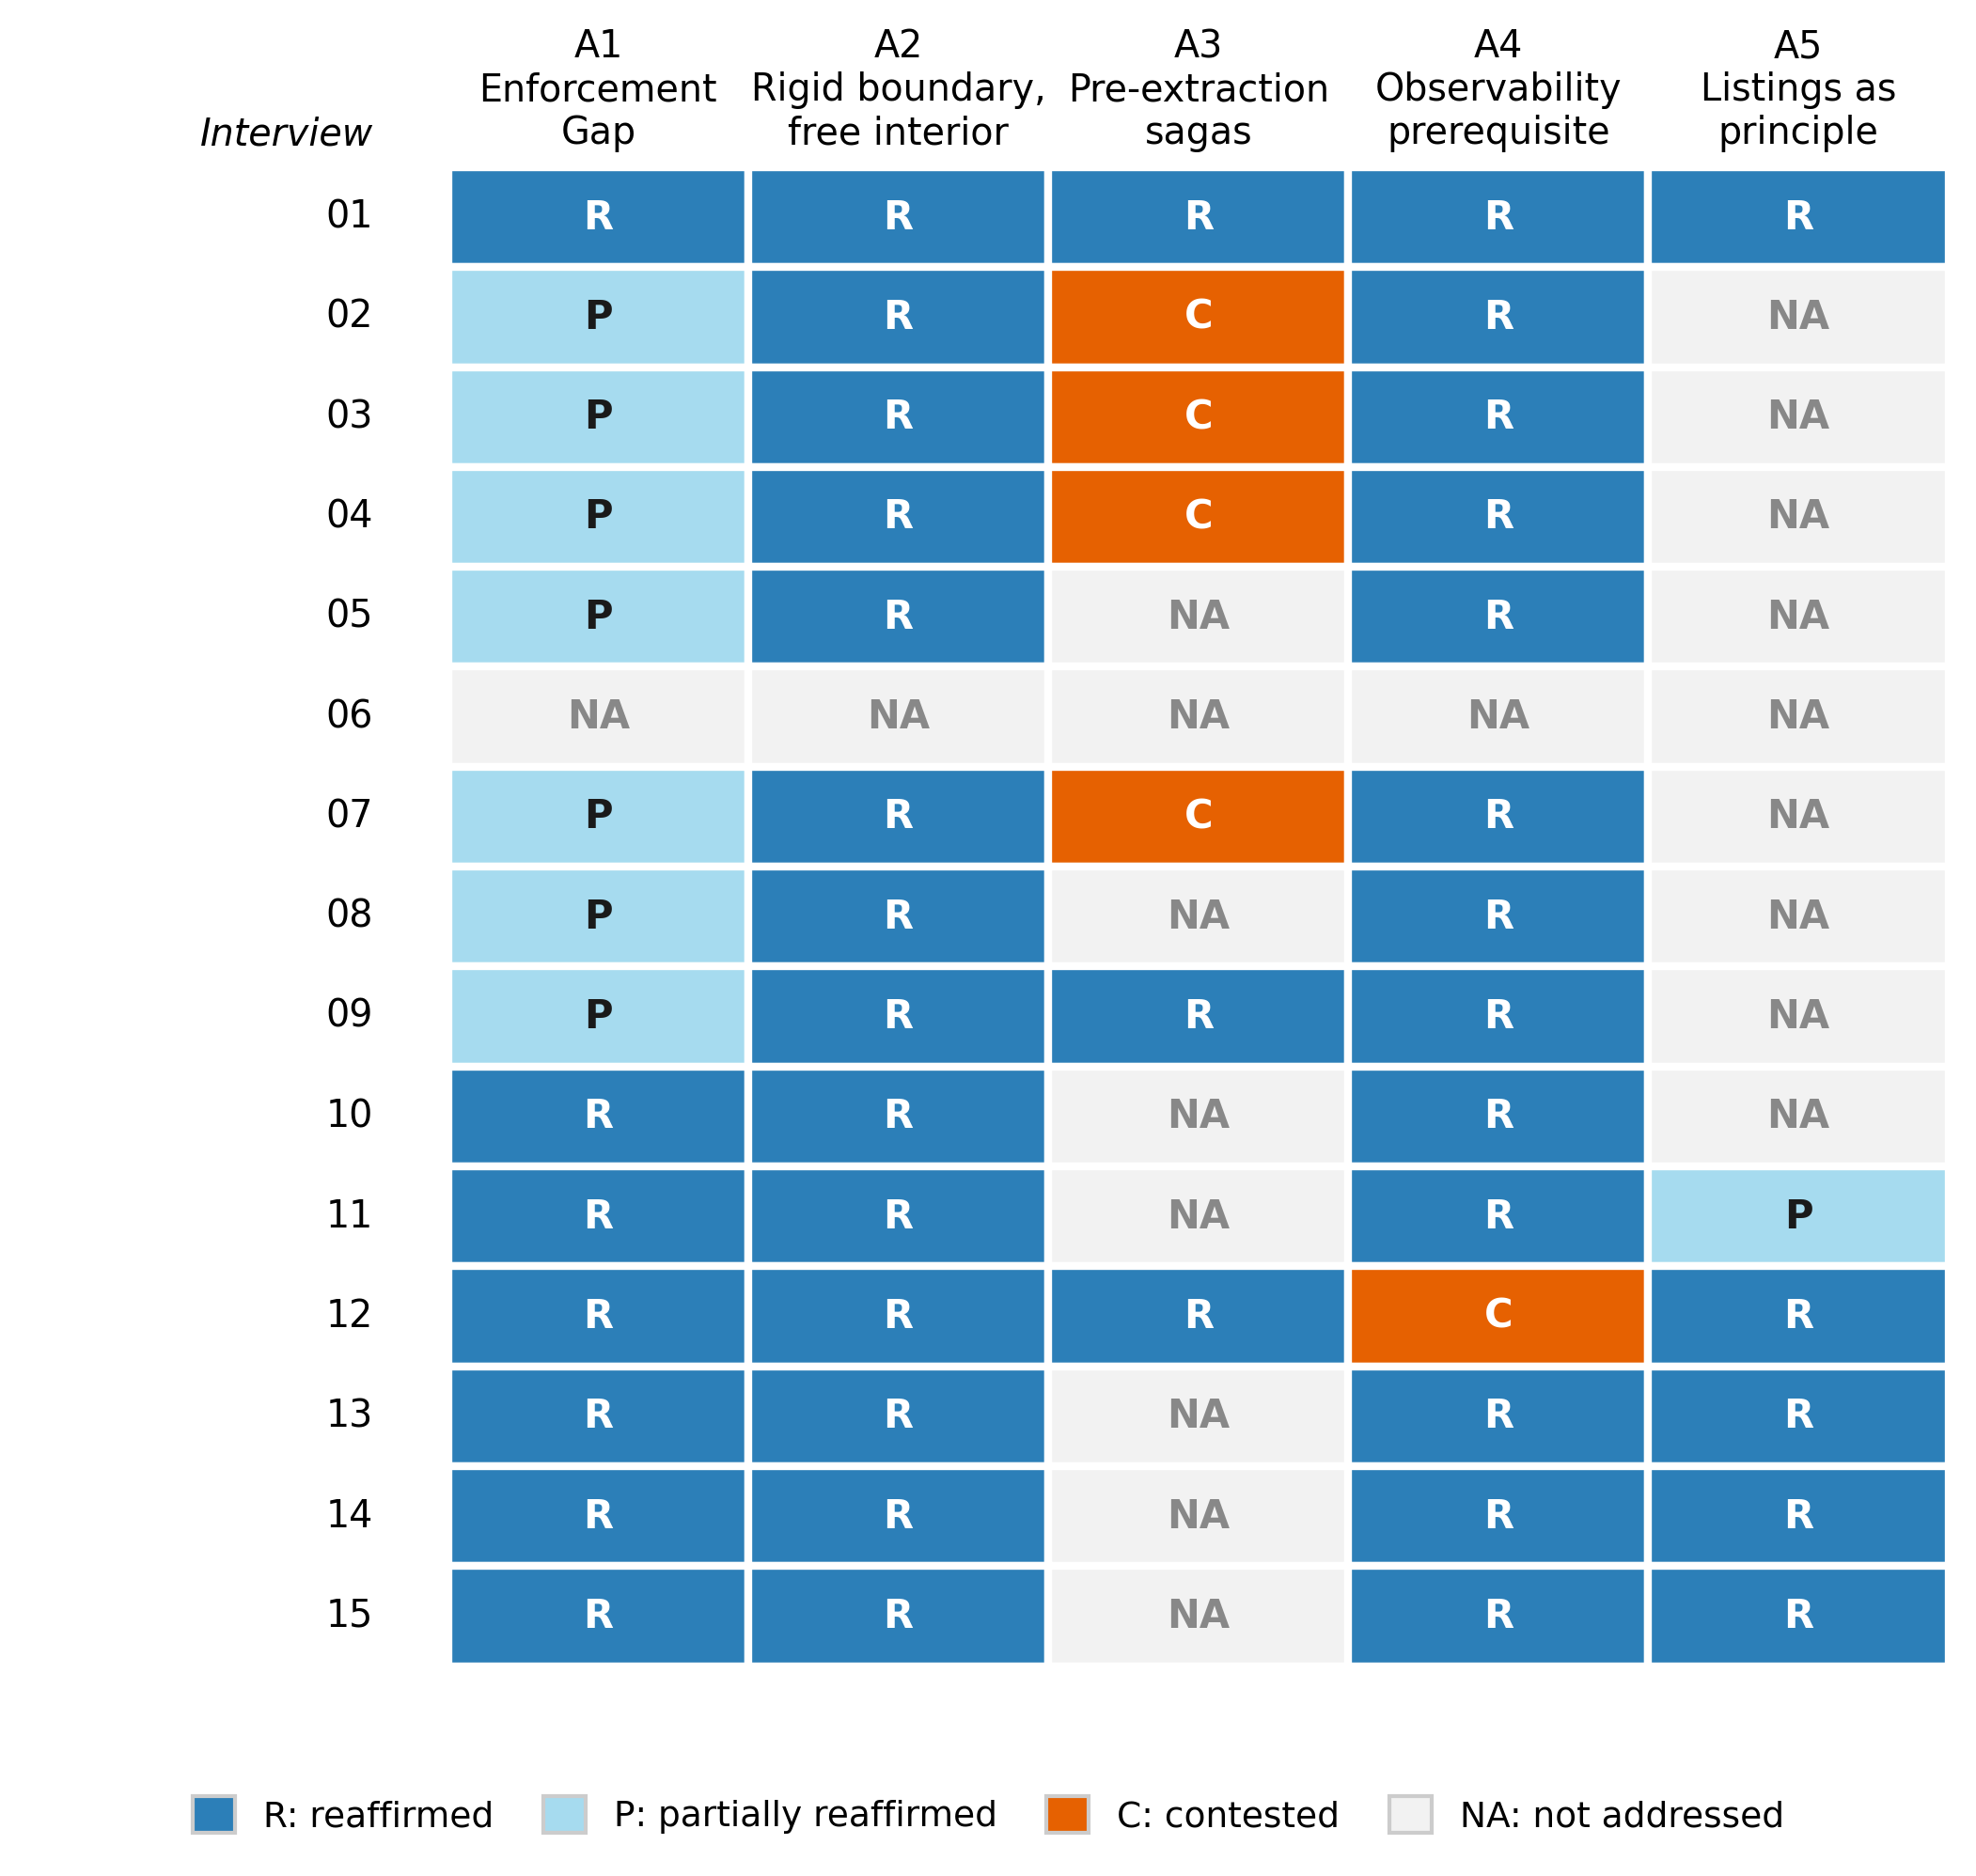
\includegraphics[width=0.88\textwidth]{ApeA/interviews_axes.png}
  \caption{Status of the five saturation axes per session}
  \label{fig:interviews-axes}
\end{figure}

Four rows deserve comment:

\begin{enumerate}[itemsep=8pt,topsep=2pt]
  \item \emph{Interview 01.} This is the session from which the five axes were declared, so its row records the original articulation rather than a reaffirmation.
  \item \emph{Interview 06.} The session did not probe the axes, consistent with its advisory character.
  \item \emph{Interview 09.} The session reaffirmed A3 by defending sagas as immediate value, against the contesting pattern of Interviews 02, 03, 04, and 07.
  \item \emph{Interview 12.} The session reaffirmed A3 conditional on a working saga boilerplate and contested A4 on timing grounds, arguing that the observability investment is premature for early-stage systems.
\end{enumerate}

The cross-series reading of the figure matches the synthesis reported in Chapter~\ref{sec:conclusion}:

\begin{enumerate}[itemsep=8pt,topsep=2pt]
  \item \emph{A1 Enforcement Gap.} The axis migrated from partial reaffirmations (substance without the term) in the early sessions to strong reaffirmations from Interview 10 onward.
  \item \emph{A2 Rigid boundary, free interior.} The axis was reaffirmed in every session that addressed it.
  \item \emph{A3 Pre-extraction sagas.} This is the only contested axis, with four contesting voices, two defending or conditional voices, and the remainder silent.
  \item \emph{A4 Observability prerequisite.} This is the most consolidated axis, reaffirmed in every session that addressed it except the timing-based contestation of Interview 12.
  \item \emph{A5 Listings as principle.} The axis was unaddressed by the early sessions and consistently reaffirmed from Interview 11 onward.
\end{enumerate}

The two-consecutive-sessions criterion declared in Appendix~\ref{ape:methodology} was not met during the series, so saturation is reported as a property of the series in the conclusions chapter, not claimed from any single session.
.
%% Consolidates the session metadata, interviewee attribution, dimension
%% coverage, and saturation-axis status of the fifteen interview reports.

\section{Series overview}
\label{sec:interviews-overview}

This chapter presents the fifteen expert interview reports of the verification phase. The methodology, the seven-question protocol, and the analysis framework are consolidated in Appendix~\ref{ape:methodology}. All sessions were remote synchronous video calls, recorded and transcribed, with verbal consent captured on record, and all were conducted in Brazilian Portuguese: quotations in the per-interview sections preserve the original wording, followed by an English translation for the reader.

This overview consolidates the descriptive information that is common to every report: session metadata (Table~\ref{tab:interviews-metadata}), interviewee attribution (Table~\ref{tab:interviews-attribution}), coverage of the four evaluation dimensions (Figure~\ref{fig:interviews-dimensions}), and the cross-series status of the five saturation axes (Figure~\ref{fig:interviews-axes}). The per-interview sections that follow keep the analytical content of each session: the three strongest themes, the verbatim quote worth preserving, the coded findings with their literature-gap mapping, the post-interview questionnaire findings, the session-specific limitations, the contributions to the conclusions chapter, and a concluding remark.

\subsection*{Session metadata}

Table~\ref{tab:interviews-metadata} records the date and the total recording length of each session.

\begin{longtable}{c l l}
\caption{Session metadata of the fifteen interviews.}
\label{tab:interviews-metadata}\\
\toprule
\textbf{Interview} & \textbf{Date (2026)} & \textbf{Recording} \\
\midrule
\endhead
\bottomrule
\endfoot
01 & 29 May & approx.\ 99 min \\
02 & 1 June & approx.\ 68 min \\
03 & 1 June & approx.\ 50 min \\
04 & 1 June & approx.\ 71 min \\
05 & 2 June & approx.\ 62 min \\
06 & 2 June & approx.\ 45 min \\
07 & 3 June & approx.\ 80 min \\
08 & 5 June & approx.\ 58 min \\
09 & 6 June & approx.\ 76 min \\
10 & 8 June & 56 min \\
11 & 8 June & 65 min \\
12 & 8 June & approx.\ 42 min \\
13 & 10 June & approx.\ 46 min \\
14 & 9 June & 37 min \\
15 & 9 June & approx.\ 29 min \\
\end{longtable}

Four sessions declared an analytical cutoff, the timestamp after which the conversation leaves research-relevant content; material after the cutoff does not appear in any derived artifact. The excluded segments are administrative or post-closing conversation:

\begin{enumerate}[itemsep=8pt,topsep=2pt]
  \item \emph{Interview 01, cutoff at 01:14:43.} A confirmation-letter discussion and employer-proprietary tool demos.
  \item \emph{Interview 02, cutoff at 01:07:25.} A product brainstorm derived from the maturity matrix discussion.
  \item \emph{Interview 03, cutoff at 00:49:40.} Defense logistics and prior-interview commentary.
  \item \emph{Interview 09, cutoff at 01:14:00.} Scheduling updates without analytical material.
\end{enumerate}

The remaining eleven sessions were research-relevant in full.

\subsection*{Interviewee attribution}

Table~\ref{tab:interviews-attribution} consolidates the attribution of the fifteen participants under the \emph{Interviewee N} scheme declared in Appendix~\ref{ape:methodology}. Personal identifiers are withheld in all cases, and the reports disclose the employment context at three levels: Interviews 01 to 07 name the industry but not the employer, Interviews 08, 10, 11, and 12 name previous employers and keep the current one undisclosed, and Interviews 09, 13, 14, and 15 withhold the organization entirely (the three public-sector participants work at a Brazilian state-owned information technology company, named only by category).

\begin{longtable}{c p{6.0cm} p{4.6cm} c}
\caption{Interviewee attribution across the series.}
\label{tab:interviews-attribution}\\
\toprule
\textbf{Interview} & \textbf{Role and context} & \textbf{Education} & \textbf{XP (yrs)} \\
\midrule
\endhead
\bottomrule
\endfoot
01 & Principal Software Engineer, U.S.\ telecommunications & BSc Information Technology & 16 \\
02 & Senior Engineering Manager, U.S.\ SaaS (home services) & Dipl\^ome d'Ing\'enieur, ENSIIE (France) & 15 \\
03 & CTO across Brazilian startups & BSc Information Technology & 14 \\
04 & Engineering Manager, Australian software company; former consultant & not declared & 15 \\
05 & Principal Software Engineer, Brazilian edtech & PhD student, Software Engineering & 17 \\
06 & Adjunct professor, federal Brazilian university & PhD Computer Science (2016) & n/d \\
07 & Engineering Manager, Brazilian fintech & BSc Information Systems & 12 \\
08 & Principal Software Engineer, formerly at Shopify & Engineering degree & 10+ \\
09 & Software engineer, distributed and modular monolith systems & Dipl\^ome d'Ing\'enieur, \'Ecole Polytechnique; BEng Poli-USP & 4 \\
10 & Senior Software Engineer, formerly at GitHub and Red Hat & Engineering degree & 14 to 15 \\
11 & Software engineer, formerly at Samsung SRBR, Ita\'u, Viva Real & MSc Computer Science, UFAM & 10+ \\
12 & Backend Software Engineer, formerly at VR Benef\'icios and Ambev & Technologist, Systems Analysis, IFSP & 7 \\
13 & Engineering Manager, state-owned IT company (public sector) & MSc UFMG; doctoral student & 13 \\
14 & Software Engineer, state-owned IT company (public sector) & BSc Computer Science, UniBH & 10 \\
15 & Systems Analyst, state-owned IT company (public sector) & Technologist, Systems Analysis, Una & 13 \\
\end{longtable}

The profile categories tracked across the series are eleven industry practitioners, three mixed industry-and-academic profiles (Interviews 05, 11, and 13), and one academic researcher (Interview 06). The sample covers Brazilian, Australian, French, and United States contexts, with years of professional experience from four to seventeen.

\subsection*{Coverage of the four evaluation dimensions}

Figure~\ref{fig:interviews-dimensions} shows how thoroughly each session covered the four evaluation dimensions: D1 Architectural Design, D2 Operational Fit, D3 Organizational Alignment, and D4 Guideline Orientation. The cells use five markers: \emph{D} for covered with depth, \emph{B} for covered with breadth or covered more briefly, \emph{O} for addressed organically (the participant raised the dimension without prompting), \emph{I} for addressed implicitly or indirectly, and \emph{NA} for not addressed.

\begin{figure}[htb]
  \centering
  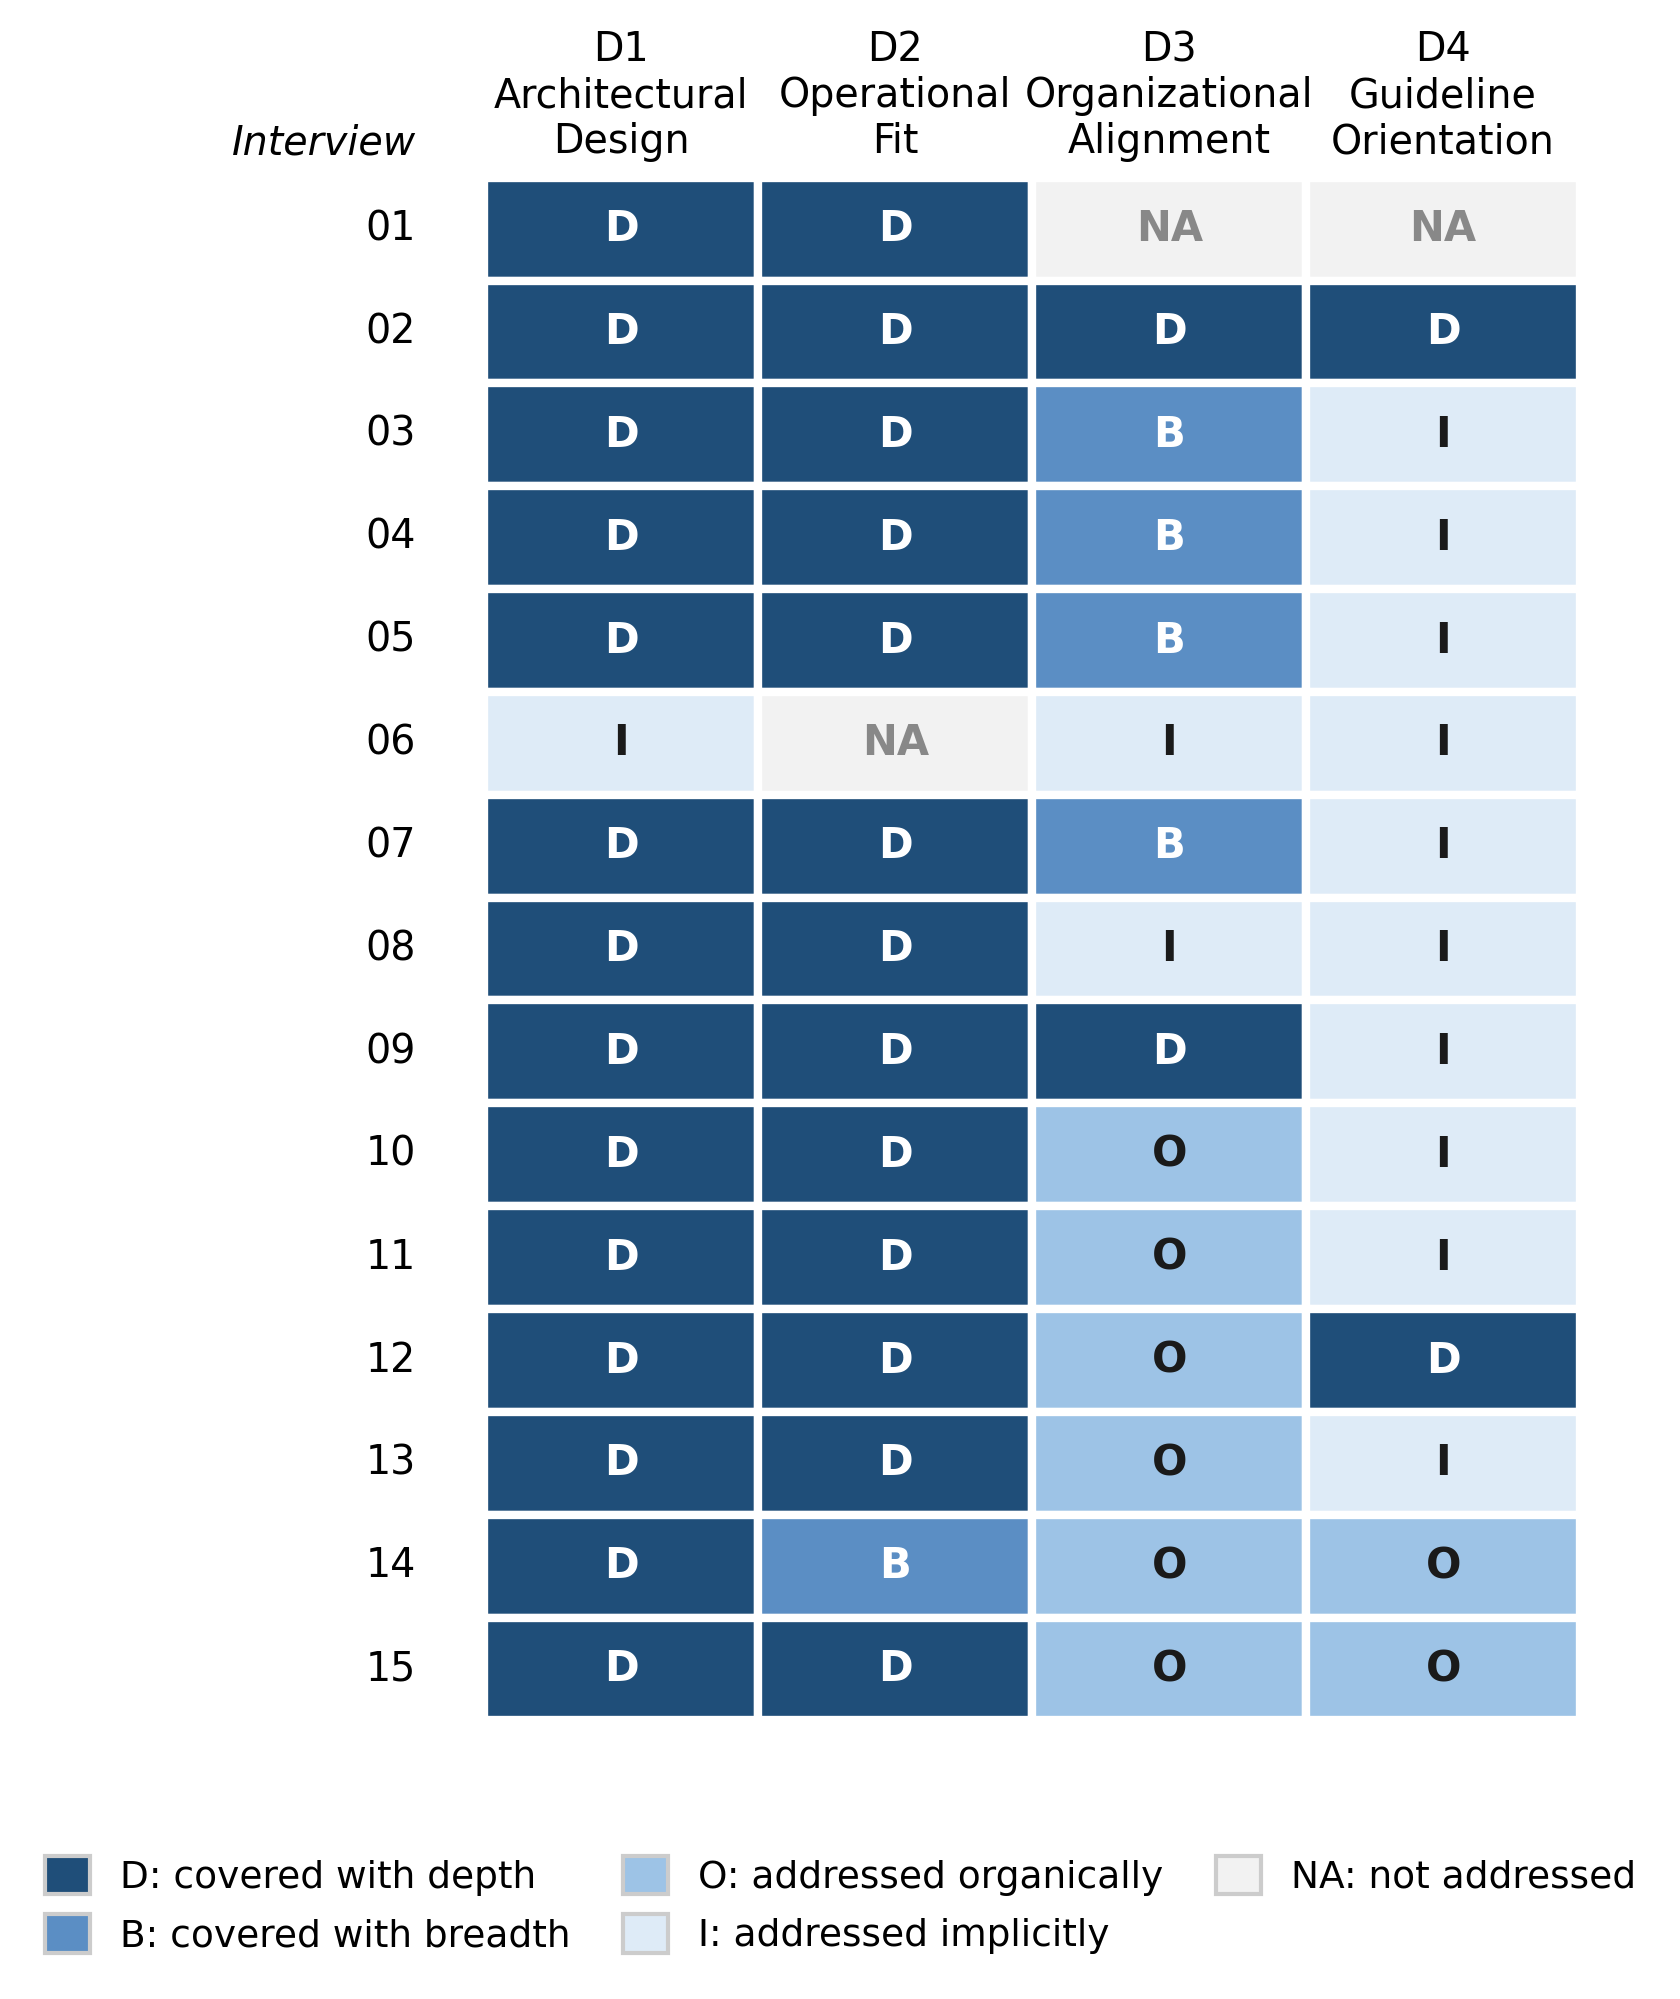
\includegraphics[width=0.78\textwidth]{ApeA/interviews_dimensions.png}
  \caption{Coverage of the four evaluation dimensions per session}
  \label{fig:interviews-dimensions}
\end{figure}

Two rows deserve comment:

\begin{enumerate}[itemsep=8pt,topsep=2pt]
  \item \emph{Interview 01.} The session used an earlier thirty-question script that produced the declared coverage gaps in D3 and D4; the protocol was revised to seven questions with one reserved for the deferred dimensions, and no subsequent session reproduced the gap.
  \item \emph{Interview 06.} The session focused on historical precedent and methodological advice rather than on probing the guidelines directly, which explains its lighter row.
\end{enumerate}

\subsection*{Saturation axes across the series}

Figure~\ref{fig:interviews-axes} consolidates the status of the five saturation axes tracked since Interview 01: A1 the spontaneous articulation of the Enforcement Gap, A2 the rigid-boundary and free-interior distinction, A3 pre-extraction sagas as actual practice, A4 observability as a systemic prerequisite, and A5 the reading of code listings as principle rather than prescription. The cells use four markers: \emph{R} for reaffirmed (fully or with a refinement), \emph{P} for partially reaffirmed (the substance was articulated without the named concept), \emph{C} for contested, and \emph{NA} for not addressed.

\begin{figure}[htb]
  \centering
  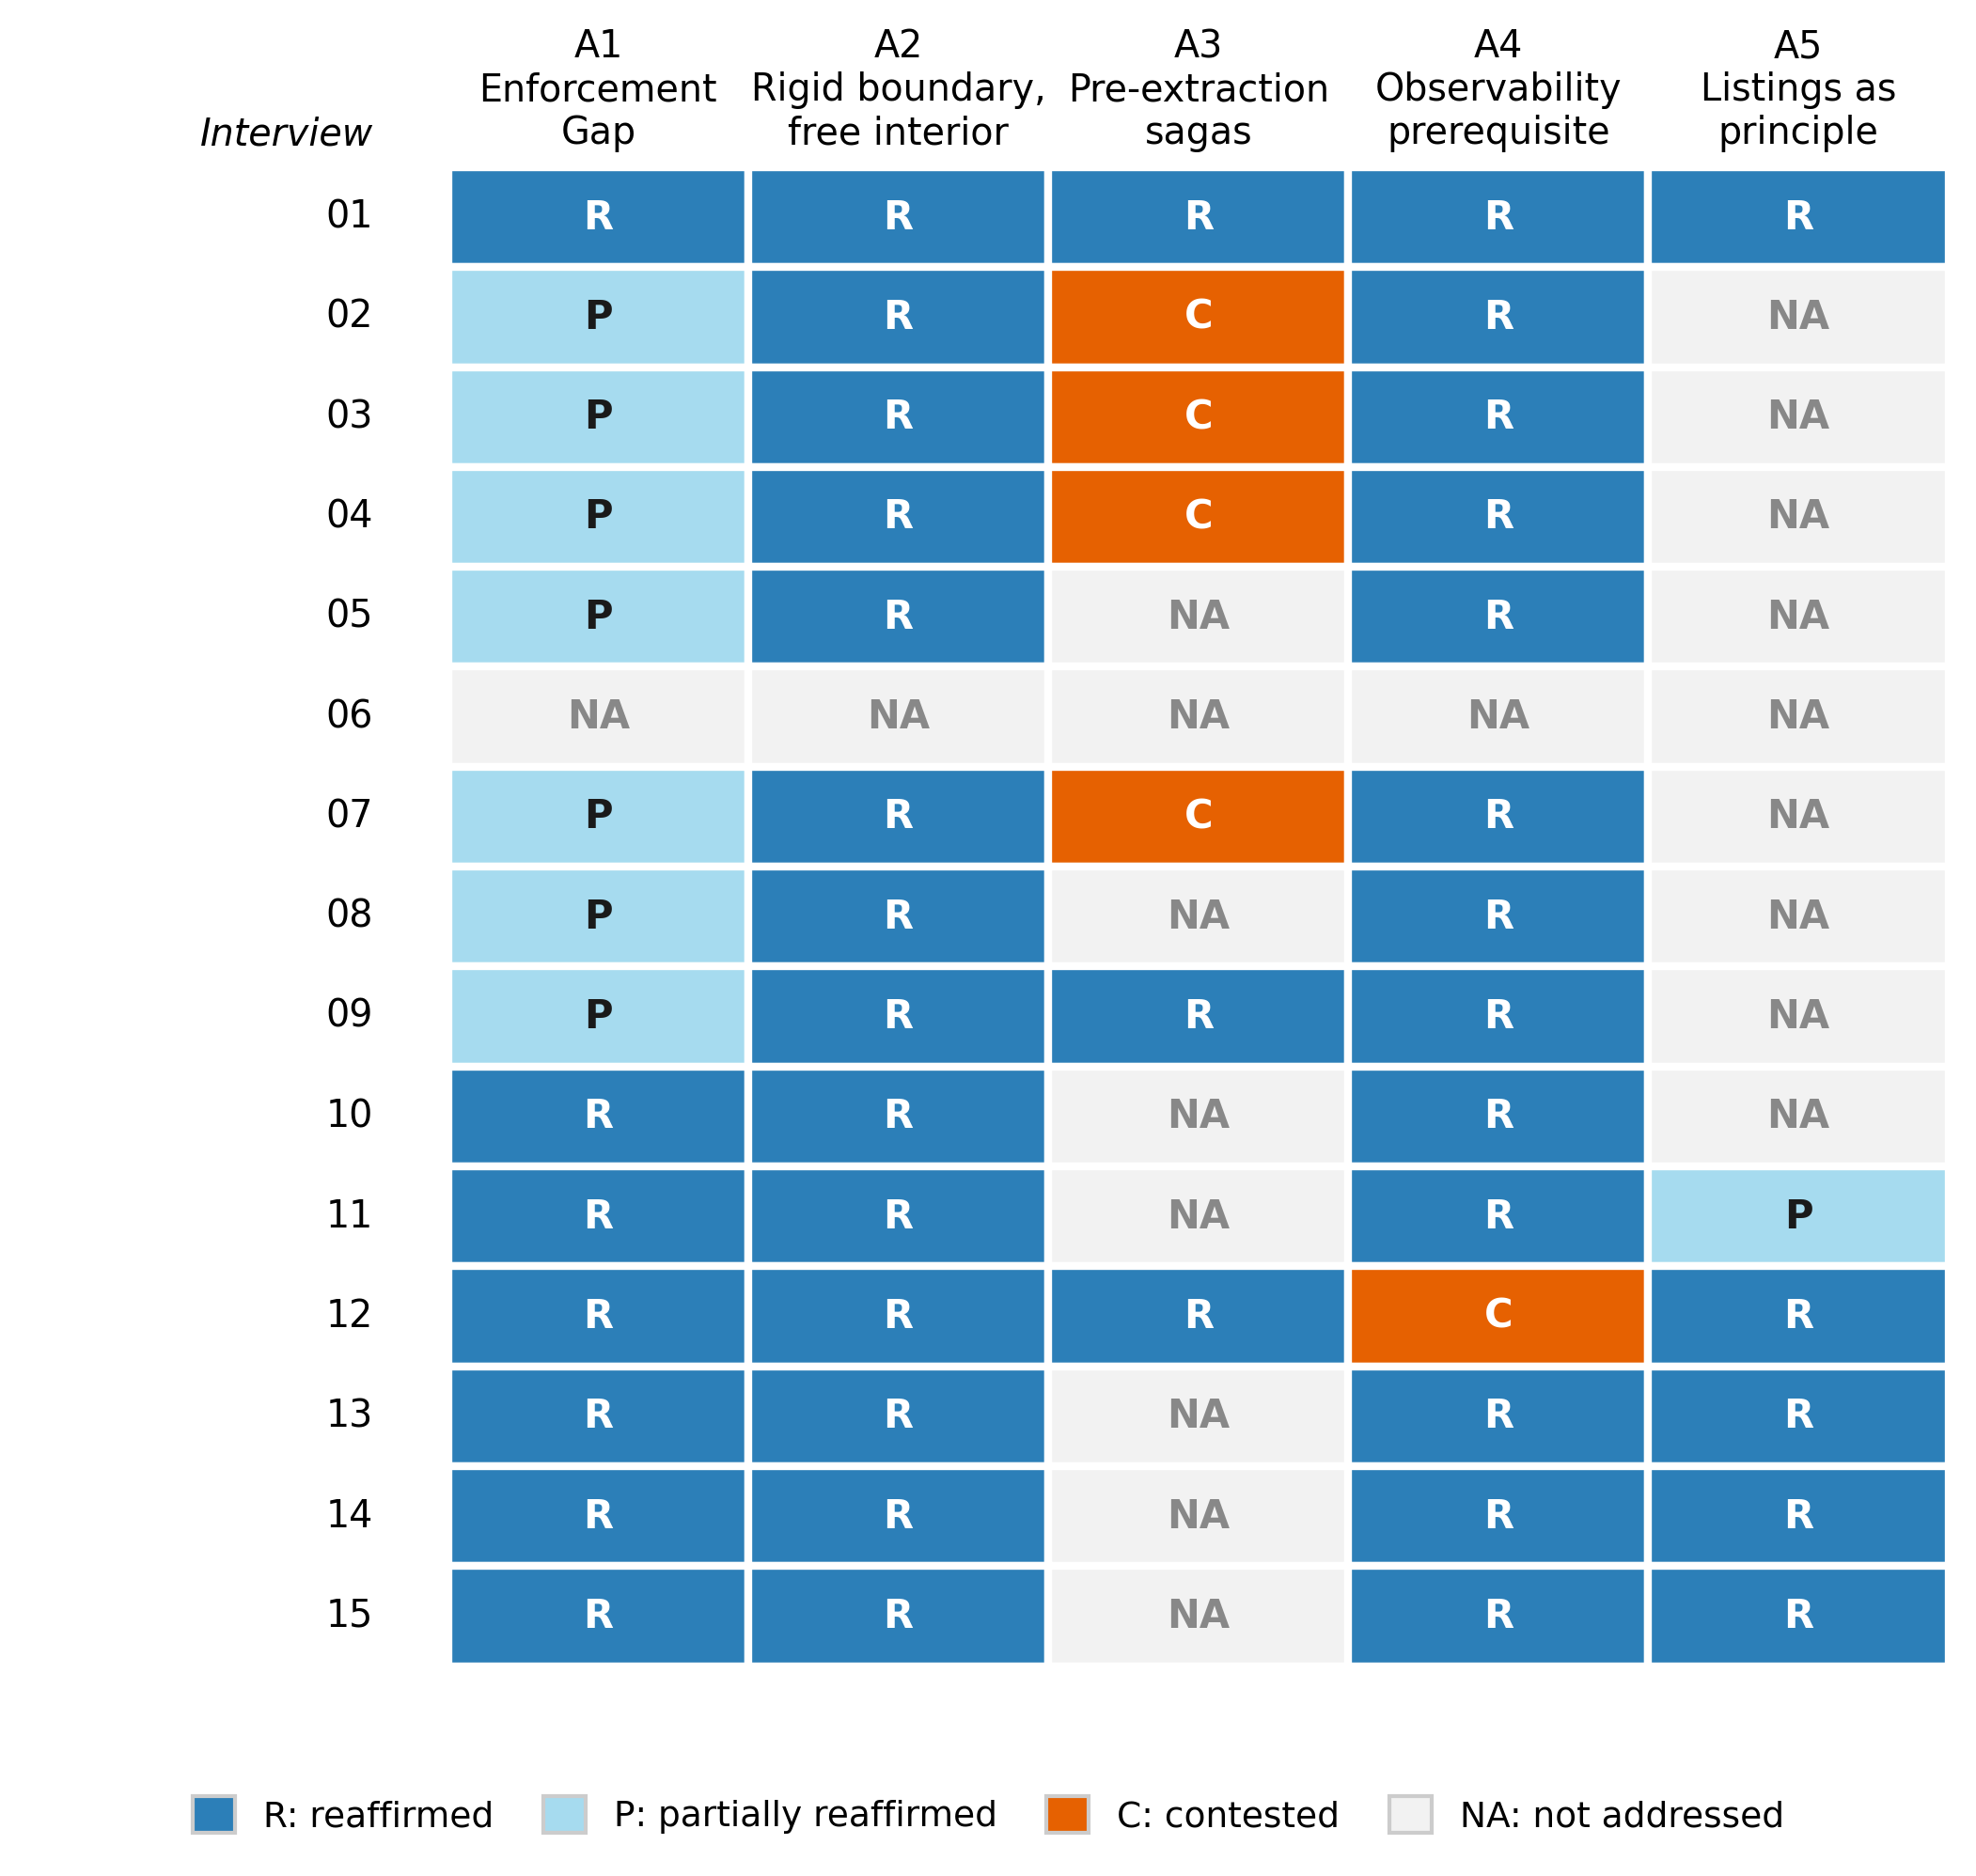
\includegraphics[width=0.88\textwidth]{ApeA/interviews_axes.png}
  \caption{Status of the five saturation axes per session}
  \label{fig:interviews-axes}
\end{figure}

Four rows deserve comment:

\begin{enumerate}[itemsep=8pt,topsep=2pt]
  \item \emph{Interview 01.} This is the session from which the five axes were declared, so its row records the original articulation rather than a reaffirmation.
  \item \emph{Interview 06.} The session did not probe the axes, consistent with its advisory character.
  \item \emph{Interview 09.} The session reaffirmed A3 by defending sagas as immediate value, against the contesting pattern of Interviews 02, 03, 04, and 07.
  \item \emph{Interview 12.} The session reaffirmed A3 conditional on a working saga boilerplate and contested A4 on timing grounds, arguing that the observability investment is premature for early-stage systems.
\end{enumerate}

The cross-series reading of the figure matches the synthesis reported in Chapter~\ref{sec:conclusion}:

\begin{enumerate}[itemsep=8pt,topsep=2pt]
  \item \emph{A1 Enforcement Gap.} The axis migrated from partial reaffirmations (substance without the term) in the early sessions to strong reaffirmations from Interview 10 onward.
  \item \emph{A2 Rigid boundary, free interior.} The axis was reaffirmed in every session that addressed it.
  \item \emph{A3 Pre-extraction sagas.} This is the only contested axis, with four contesting voices, two defending or conditional voices, and the remainder silent.
  \item \emph{A4 Observability prerequisite.} This is the most consolidated axis, reaffirmed in every session that addressed it except the timing-based contestation of Interview 12.
  \item \emph{A5 Listings as principle.} The axis was unaddressed by the early sessions and consistently reaffirmed from Interview 11 onward.
\end{enumerate}

The two-consecutive-sessions criterion declared in Appendix~\ref{ape:methodology} was not met during the series, so saturation is reported as a property of the series in the conclusions chapter, not claimed from any single session.
